\begin{section}{Lokales Differenzieren}\index{Differenzieren!lokal}
\begin{subsection}{Die mittlere Änderungsrate}
\begin{defi}{Die mittlere Änderungsrate}{maer}\index{Änderungsrate!mittlere}
Der Quotient $$\dfrac{\Delta y}{\Delta x} = \dfrac{f(b) - f(a)}{b - a}$$ heißt mittlere Änderungsrate oder Differenzenquotient der Funktion f im Intervall $\left[a;b\right]$.\\
Die geometrische Deutung des Differenzenquotient \index{Änderungsrate!Differenzenquotient} ist die Steigung der Sekante durch die Punkte $P(a|f(a))$ und $Q(b|f(b))$ am Graphen $G_f$ der Funktion $f$.
\end{defi}
\begin{bsp}{Ein Beispiel für die mittlere Änderungsrate}{bspmaer}
Gegeben sind die Punkte $P(3|4)$ und $Q(6|1)$ auf dem Graphen $G_f$ einer Funktion $f$. Die mittlere Änderungsrate bestimmt sich damit wie folgt: $$ \dfrac{\Delta y}{\Delta x} = \dfrac{4-1}{3-6} = \dfrac{3}{-3} = -1$$
\end{bsp}
\begin{bsp}{Graphische Darstellung der Sekantensteigung}{}
Gegeben ist die Funktion $f(x) =\dfrac{1}{2}x^3-x^2-2x +1$ mit $\mathds{D}_f =\mathds{R}$ und die Punkte $P(1|-1,51)$ und $Q(3,3|1,48)$. Um die mittlere Änderungsrate zu bestimmen muss jetzt die Steigung der Sekante durch die Punkt $P$ und $Q$ berechnet werden.
$$m=\dfrac{\Delta y}{\Delta x} = \dfrac{y_2 -y_1}{x_2 -x_1} = \dfrac{1,48 -(-1,51)}{3,3 -1} = \dfrac{2,99}{2,3} = \dfrac{13}{10} = 1,3 $$
\begin{center}
\begin{tikzpicture}
\begin{axis}[xmin= -3.5, xmax = 4.5, ymin= -4, ymax= 4,
        axis lines = middle, 
         x=1cm,y=1cm,
        ymajorgrids=true,
        xmajorgrids=true,
        xtick={-3, -2, -1, 0, ..., 4},
        ytick={-4, -3, -2, ..., 3},
        xlabel = $x$,
        ylabel=$y$]
            \addplot[color= black, samples = 300, domain= -2:3.5]{0.5*x^3-x^2-2*x^1 +1};
            \draw[color = red] (3,2.5) node[left] {$G_f$};
          \addplot[color= red, samples = 300, domain= -1:4]{1.3*x -2.81};
           \draw[color = red] (1,-3.5) node {Sekante};
           \draw (1,-1.51)-- ++(-2.5pt,-2.5pt) -- ++(5pt,5pt) ++(-5pt,0pt) -- ++(5pt,-5pt) node[left] {P};
           \draw (3.3,1.48)-- ++(-2.5pt,-2.5pt) -- ++(5pt,5pt) ++(-5pt,0pt) -- ++(5pt,-5pt) node[right] {Q};
           
            \draw[color = red] (2.2,0.5) node[left] {$\dfrac{\Delta y}{\Delta x} = 1,3$};
\end{axis}
\end{tikzpicture}
\end{center}
\end{bsp}
\end{subsection}
\subsection{Definition der Ableitung}
Die mittlere Änderungsrate beschreibt die durchschnittliche Steigung des Graphen einer Funktion zwischen zwei bestimmten Punkten. Die Ableitung realisiert den Übergang von der Sekante zur Tangente.
\begin{merke}{Der Grenzwert einer Funktion}{}
\index{Ableitung!Definition}
\begin{itemize}
 \item Nähern sich die Funktionswerte $f(x)$ einer Funktion $f$ an der Stelle $x_0$ einer Zahl $a$ beliebig genau an, das ist der Fall wenn sich die Werte für $x$ von links und von rechts an $x_0$ beliebig genau annähern, so heißt $a$ Grenzwert der Funktion $f(x)$. \\Kurzschreibweise: $$\lim_{x \rightarrow x_0} f(x)= a$$ 
 \item Der Punkt Q laufe auf einer Kurve von links und rechts auf den Punkt P zu. Ergibt sich dabei ein gemeinsamer Grenzwert der Sekante, heißt die Grenzgerade Tangente an die Kurve im Punkt P.
 \item Die Steigung eines Graphen im Punkt P ist gleich der Steigung der Tangente in diesem Punkt.
\end{itemize}
\end{merke}
Um die Ableitung zu definieren, betrachten wir als Beispiel die Normalparabel mit der Gleichung $$ y=x^2 $$ und darauf einen Punkt $P(1,5|2,25)$. Zur Bestimmung der Sekantensteigung bildet man den Differenzenquotienten zwischen dem Punkt $P$ und einem weiteren beliebigen Punkt $Q(x|x^2)$. 
\begin{bem*}{Differenzenquotient für $f(x) =x^2 $}\index{Änderungsrate!Differenzenquotient}
  
  $$ m_s(x)= \dfrac{\Delta y}{\Delta x} = \dfrac{f(x) - 2,25}{x - 1,5} = \dfrac{x^2 - 2,25}{x- 1,5} = \dfrac{(x-1,5)(x+1,5)}{x-1,5} =x+1,5 $$
Nähert sich der Punkt $Q$ beliebig nahe an den Punkt $P$ an, so unterscheidet sich die Steigung der Sekante immer weniger von 3. Man spricht in diesem Fall auch von einem Grenzwert.
$$\lim_{x\rightarrow 1,5} m_s(x) = 3$$
\end{bem*}

\label{hmethode}
\begin{merke*}{Die h-Methode zur Berechnung der Steigung }{}\index{Ableitung!h-Methode}
Es wird eine Hilfsvariable h eingeführt, diese gibt die Abweichung der Koordinate $x$ von der Koordinate $x_0$ an. Damit gilt $x=x_0 + h$. Mit dieser Definition der Stelle $x$ ist es nun möglich den Grenzwert an einer beliebigen Stelle $x_0$ aufzustellen: $$m_t =\lim_{h\rightarrow 0} m_t(x_0 +h) =\lim_{h\rightarrow 0} \dfrac{f(x_0 + h) - f(x_0)}{h}.$$
\end{merke*}
\begin{defi}{Differentialquotiont oder Ableitung}{} \index{Ableitung!Definition}
    Der Grenzwert des Differenzenquotienten $\frac{\Delta y}{\Delta x}$ für $x\rightarrow x_0$ heißt Differentialquotient oder Ableitung der Funktion $f$ an der Stelle $x_0$ und wird mit $f'(x_0)$ bezeichnet. Es gilt der Zusammenhang:$$f'(x_0) = \lim_{x\rightarrow x_0} \dfrac{f(x) - f(x_0)}{x - x_0} = \lim_{h\rightarrow 0} \dfrac{f(x_0 +h) - f(x_0)}{h}$$
\end{defi}
\begin{bem*}{Ableitungen von Funktionen}{}
Mit Hilfe der h-Methode ist es damit möglich die Ableitung jeder Funktion an einer beliebigen Stelle $x_0$ zu bilden. Man spricht in diesem Zusammenhang dann von der ersten Ableitung der Funktion $f$ an der Stelle $x_0$.
\end{bem*}
\begin{bsp}{Graphische Interpretation der h-Methode}{}
Gegeben ist der Graph $G_f$ einer Funktion $f$ und die beiden beliebigen Punkte $P(x_0|f(x_0))$ und $Q(x_0+h|f(x_0+h))$. Durch $P$ und $Q$ verläuft eine Sekante am Graphen $G_f$. Der Abstand der beiden Punkte läuft bei der h-Methode gegen Null. 
  \begin{center}
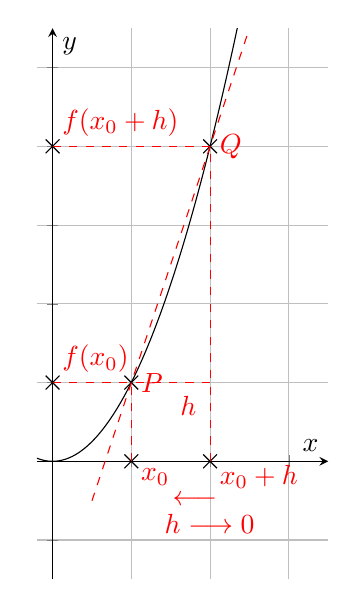
\begin{tikzpicture}
\begin{axis}[xmin= -0.2, xmax = 3.5, ymin= -1.5, ymax= 5.5,
 x=1cm,y=1cm,
        axis lines = middle, 
        ymajorgrids=true,
        xmajorgrids=true,
        xticklabels=\empty,
        yticklabels=\empty,
        xlabel = $x$,
        ylabel=$y$]  
        \addplot[color= black, samples = 300, domain= -2:2.5]{x^2};
        \draw[color= red] (1,-0.2) node[right] {$x_0$};
        \draw (1,0)-- ++(-2.5pt,-2.5pt) -- ++(5pt,5pt) ++(-5pt,0pt) -- ++(5pt,-5pt);
        \draw[color= red] (2,-0.2) node[right] {$x_0 +h$};
        \draw (2,0)-- ++(-2.5pt,-2.5pt) -- ++(5pt,5pt) ++(-5pt,0pt) -- ++(5pt,-5pt);
        \draw[color= red] (0,1.3) node[right] {$f(x_0)$};
        \draw (0,1)-- ++(-2.5pt,-2.5pt) -- ++(5pt,5pt) ++(-5pt,0pt) -- ++(5pt,-5pt);
        \draw[color= red] (0,4.3) node[right] {$f(x_0 + h)$};
        \draw (0,4)-- ++(-2.5pt,-2.5pt) -- ++(5pt,5pt) ++(-5pt,0pt) -- ++(5pt,-5pt);
         \draw[color= red] (2,4) node[right] {$Q$};
        \draw (2,4)-- ++(-2.5pt,-2.5pt) -- ++(5pt,5pt) ++(-5pt,0pt) -- ++(5pt,-5pt);
         \draw[color= red] (1,1) node[right] {$P$};
        \draw (1,1)-- ++(-2.5pt,-2.5pt) -- ++(5pt,5pt) ++(-5pt,0pt) -- ++(5pt,-5pt);
            \draw[red, dashed] (0,1 )-- (2,1);
            \draw[red, dashed] (2,0) -- (2,4);
            \draw[red, dashed] (0,4) -- (2,4);
            \draw[red, dashed] (1,0) -- (1,1);
         \draw[color= red] (1.5,0.7) node[right] {$h$};
         \addplot[color= red,dashed, samples = 300, domain= 0.5:2.5]{3*x - 2};
         \draw[red] (1.4,-0.5) node[right] {$\longleftarrow$};
         \draw[red] (1.3,-0.8) node[right] {$h\longrightarrow 0$};
\end{axis}
\end{tikzpicture}
\end{center}
 Das bedeutet, dass sich die beiden Punkten der Sekante beliebig genau annähern, ihr Abstand geht damit gegen Null ($h\rightarrow 0$). Somit wird aus der Sekannte eine Tangente.
\end{bsp}
\index{Änderungsrate!lokale}
\begin{bem*}{Tangentensteigung}{}
   Die Ableitung $f'(x_0)$ entspricht der Steigung der Tangente am Graphen von $f$ an der Stelle $x_0$. Dabei ist die Ableitung ein Maß dafür, wie stark sich die Funktionswerte in einer Umgebung um die Stelle $x_0$ ändern. \\
   Bei zeitlichen  Vorgängen spricht man von einer \textcolor{red}{momentanen Änderungsrate}, bei anderen Vorgängen von einer \textcolor{red}{lokalen Änderungsrate}.
\end{bem*}
\index{Änderungsrate!Steigungswinkel}
\index{Steigungswinkel}
\begin{bem*}{Der Steigungswinkel}{}
Der \textcolor{red}{Steigungswinkel} $\alpha$ einer Tangente ist der \textcolor{red}{spitze} Winkel zur x-Achse. Der Tangens des Steigungswinkels $\alpha$ ist gleich der Steigung $m$:$$\tan{(\alpha)} = m$$ \begin{center}
    bzw.
\end{center} $$\alpha = \arctan{(m)} = \tan^{-1}{(m)}$$
ist $m$ positiv, ist $\alpha$ positiv; ist $m$ negativ, ist $\alpha$ negativ. 
\begin{center}
\begin{tikzpicture}
\begin{axis}[xmin= -2, xmax = 3.5, ymin= -1.5, ymax= 3.5,
 x=1cm,y=1cm,
        axis lines = middle, 
        xticklabels=\empty,
        yticklabels=\empty,
        xlabel = $x$,
        ylabel=$y$]
        \addplot[red, samples = 100]{x^3+1};
        \addplot[blue, samples = 100]{3*x-1};
        \draw[color= red] (0.5,2) node {$P$};
          \draw (1,2)-- ++(-2.5pt,-2.5pt) -- ++(5pt,5pt) ++(-5pt,0pt) -- ++(5pt,-5pt);

          \draw (1,0) coordinate (a) -- (0.33,0) coordinate (b) -- (1,2) coordinate (c)  pic[ draw = blue, fill = red!25!white, ->, angle eccentricity =1.2, angle radius = 1cm] {angle = a--b--c};
        \draw[color= black] (1.5,0.6) node {$\alpha$};
\end{axis}
\end{tikzpicture}
\end{center}
\end{bem*}
Mit Hilfe dieser Definitionen und Überlegungen ist es nun möglich, die Steigung einer Funktion an einer bestimmten Stelle zu berechnen und den dazugehörigen Steigungswinkel der Tangente zu bestimmen. Anhand eines Beispiels wird dieses jetzt exemplarisch durchgeführt.
\begin{bsp*}{Berechnung der Steigung und Steigungswinkel}{}
Gegeben ist die Funktion $f(x)= 2x^2 - 3x +2 $ und dem Definitionsbereich $\mathds{D}_f = \mathds{R}$. Betrachtet wird die Stelle $x_0 = \dfrac{3}{2}$.\\
Vorgehen:
\begin{enumerate}
    \item Bestimmung der ersten Ableitung mit Hilfe der h-Methode
    \item Berechnung der Steigung an einer bestimmten Stell $x_0$
    \item Berechnung des Steigungswinkels der Tangente an dieser Stelle am Graphen
\end{enumerate}
Berechnung:
\begin{equation*}
\begin{split}
f'(x_0) &= \lim_{h\rightarrow 0} \dfrac{f(x_0+h)-f(x_0)}{h}\\ f'(1,5)&=\lim_{h\rightarrow 0} \dfrac{f(1,5 +h) - f(1,5)}{h}\\ &= \lim_{h\rightarrow 0} \dfrac{2\cdot (1,5 +h)^2 -3\cdot(1,5+h) + 2-(2\cdot (1,5)^2 - 3\cdot (1,5) + 2)}{h}\\
&= \lim_{h\rightarrow 0} \dfrac{2\cdot (2,25 +3h + h^2) -3\cdot(1,5+h) + 2 - (4,5 -2,25 +2)}{h}\\
&= \lim_{h\rightarrow 0} \dfrac{4,5+6h+2h^2-2,25-3h+2-(4,5 -2,25 +2)}{h}\\
&= \lim_{h\rightarrow 0} \dfrac{2h^2+3h}{h}= \lim_{h\rightarrow 0} \dfrac{h\cdot( 2h+3)}{h} = \lim_{h\rightarrow 0} 2h+3\\
&= \textcolor{red}{3 = m_T} \hspace{0.3cm} \longrightarrow \hspace{0.3cm} \textbf{Steigung der Tangente}
\end{split}
\end{equation*}

Berechnung des Steigungswinkels der Tangente an der Stelle $x=1,5 $: 
\begin{equation*}
\begin{split}
\tan{(\alpha)} &= m\\
\tan{(\alpha)} &= 3\\
\alpha &= \arctan{(3)} \approx 71,57^{\circ}  
\end{split}
\end{equation*}
\end{bsp*}
Als Beispiel für die Möglichkeiten der h-Methode werden die Ableitungen mehrerer Funktionen an einer beliebigen aber festen Stelle $x_0$ gebildet.
\begin{bsp*}{Ableitungen ausgesuchter Funktionen}{}
Im folgenden werden die Ableitungen einiger Funktionen mithilfe der h-Methode gebildet. Dabei wird eine beliebige aber feste Stelle $x_0$ verwendet.
\begin{itemize}
    \item Die konstante Funktion $f(x) = c$. \index{Ableitung!h-Methode!$f(x) =c$}
    \begin{equation*}
\begin{split}
f'(x_0)&= \lim_{h\rightarrow 0} \dfrac{f(x_0 +h) - f(x_0)}{h}\\
&= \lim_{h\rightarrow 0} \dfrac{c-c}{h} = \lim_{h\rightarrow 0} \dfrac{0}{h}  \\
 &= 0
\end{split}
\end{equation*}
\item Die lineare Funktion $f(x) = m\cdot x + t$\index{Ableitung!h-Methode!$f(x) =m\cdot x + t$}
\begin{equation*}
\begin{split}
f'(x_0)&= \lim_{h\rightarrow 0} \dfrac{f(x_0 +h) - f(x_0)}{h}\\
&= \lim_{h\rightarrow 0} \dfrac{m\cdot (x_0 + h) + t -(m\cdot x_0 +t)}{h} \\
 &=  \lim_{h\rightarrow 0} \dfrac{m\cdot x_0 + m\cdot h + t - m\cdot x_0 - t }{h} \\
 &= \lim_{h\rightarrow 0} \dfrac{m\cdot \cancel{h}}{\cancel{h}} \\
 &= \lim_{h\rightarrow 0} m = m
\end{split}
\end{equation*}
\item Die einfache gebrochen-rationale Funktion $f(x) = \dfrac{1}{x}$\index{Ableitung!h-Methode!$f(x) =\frac{1}{x}$}
\begin{equation*}
\begin{split}
f'(x_0)&= \lim_{h\rightarrow 0} \dfrac{f(x_0 +h) - f(x_0)}{h}\\
&= \lim_{h\rightarrow 0} \dfrac{\dfrac{1}{x_0 + h} -\dfrac{1}{x_0}}{h} \hspace{0.5cm} | \text{ erweitern der Brüche auf: }\hspace{0.1cm} x_0 \cdot (x_0 + h) \\
&= \lim_{h\rightarrow 0} \dfrac{\dfrac{x_0}{x_0\cdot (x_0 + h)} -\dfrac{x_0 + h}{x_0\cdot (x_0 + h)}}{h} 
= \lim_{h\rightarrow 0} \dfrac{\dfrac{x_0 - (x_0 +h)}{x_0\cdot (x_0 + h)}}{h}
= \lim_{h\rightarrow 0} \dfrac{\dfrac{x_0 - x_0 -h}{x_0\cdot (x_0 + h)}}{h}\\
&= \lim_{h\rightarrow 0} \dfrac{\dfrac{-h}{x_0\cdot (x_0 + h)}}{h} \hspace{0.5cm} | \hspace{0.5cm}\text{ Umformung des Doppelbruchs } \\
&= \lim_{h\rightarrow 0} \dfrac{-h}{h\cdot x_0\cdot (x_0 + h)}
= \lim_{h\rightarrow 0} \dfrac{-\cancel{h}}{\cancel{h}\cdot x_0\cdot (x_0 + h)}\\
&=\lim_{h\rightarrow 0} \dfrac{-1}{x_0\cdot (x_0 + h)} = \lim_{h\rightarrow 0} \dfrac{-1}{x^2_0 + x_0\cdot h}\\
&= -\dfrac{1}{x^2_0}
\end{split}
\end{equation*}
\end{itemize}
\end{bsp*}
\subsection{Differenzierbarkeit}\index{Differenzieren!Differenzierbarkeit} \index{Ableitung!Differenzierbarkeit}
\begin{defi}{Die Differenzierbarkeit einer Funktion}{}
 Eine Funktion f heißt an der Stelle $x_0$ im Inneren des Definitionsbereichs $D_f$ differenzierbar, wenn der Grenzwert \begin{equation*}
     f'(x_0) =\lim_{h\rightarrow 0}\dfrac{f(x_0 +h) -f(x_0)}{h}
 \end{equation*} existiert, sich also bei links- und rechtsseitiger Annäherung der gleiche Wert ergibt. Der Grenzwert des Differenzenquotient heißt Differentialquotient.
\end{defi}
\begin{bsp*}{Die Überprüfung der Differenzierbarkeit mit der h-Methode}\index{Differenzieren!Differenzierbarkeit!Beispiel}
    Gegeben ist die Funktion $f(x)= x^2 + |x|$, wir überprüfen die Ableitung an der Stelle $P(0|f(0))$.

$$f(x)= \begin{cases}
              x^2 + x & \text{für}\hspace{0.5cm} x\geq 0\\
              x^2 - x & \text{für}\hspace{0.5cm}  x< 0 
         \end{cases}$$
Für die Untersuchung der Differenzierbarkeit sind folgende Grenzwerte zu überprüfen::
\begin{equation*}
\begin{split}
f'(0) &= \lim_{h\rightarrow0^-} \dfrac{f(0+h)-f(0)}{h}\\ &=\lim_{h\rightarrow 0^-} \dfrac{(0+h)^2 - (0+h) -0}{h}\\ &= \lim_{h\rightarrow 0^-} \dfrac{h^2-h}{h} = \lim_{h\rightarrow 0^-} h-1=-1 
\end{split}
\end{equation*}
\begin{equation*}
\begin{split}
f'(0)&=\lim_{h\rightarrow 0^+}\dfrac{f(0+h)-f(0)}{h}\\
&=\lim_{h\rightarrow 0^+} \dfrac{(0+h)^2 + (0+h) -0}{h}\\ 
&=\lim_{h\rightarrow 0^+} \dfrac{h^2 + h}{h} = \lim_{h\rightarrow 0^+} h+1 =1
\end{split}
\end{equation*}
Der Differenzenquotient hat daher für $x\rightarrow 0$ keinen Grenzwert, die Funktion $f$ ist damit an der Stelle $x_0 = 0$ nicht differenzierbar. Der Graph $G_f$ hat an dieser Stelle einen "`Knick"'.
\end{bsp*}
\subsection{Lineare Transformation}
\begin{bem*}{}\index{Lineare Transformation}
Die Lineare Transformation der Betragsfunktion ändert nichts an der Nicht-Differenzierbarkeit der Funktion. Ein Beispiel für die Transformationen mithilfe des Betrags wird im Anhang \ref{ltbf} erläutert.
\end{bem*}
Während der letzten Schuljahre wurden verschiedene Funktionsarten einer linearen Transformation unterzogen. Als Beispiel wird hier auf die Funktionen: 
 \begin{equation*}
    \begin{split}
        f(x) &= x^2\\
        g(x) &= \sin{(x)}\\
        h(x) &= \cos{(x)}
    \end{split}
\end{equation*}
verwiesen.\\ 
In Jahrgangsstufe 9 wurde die Normalparabel auf unterschiedlichste Arten transformiert. In der 10. Jahrgangsstufe wurden Trigonometrischen Funktionen transformiert.
\begin{bsp*}{Transformationen am Bespiel der Normalparabel}{}\index{Lineare Transformation!Beispiel}
Der Graph der Funktion $f(x) = x^2$ läßt sich wie folgt transformieren:
\begin{itemize}
\item $g_1(x) = -x^2$ $\Longrightarrow$ Normalparabel an der $x-$Achse gespiegelt
\item $g_2(x) =   x^2 +a$ $\Longrightarrow$ $G_f$  Richtung der y--Achse um a verschoben
\item $g_3(x) =(x-a)^2$ $\Longrightarrow$ $G_f$ in Richtung der x--Achse um a verschoben
\item $g_4(x) =a\cdot x^2$ und $a>0$, $\Longrightarrow$ $G_f$ in Richtung der y--Achse mit dem Faktor a gestreckt bzw. gestaucht
\end{itemize}
\end{bsp*}

\begin{merke}{Allgemeine Darstellung der Linearen Transformationen} 
Die lineare Transformation lässt sich allgemein wie folgt schreiben:\index{Lineare Transformation!allgemein}\\
Wir erhalten aus dem Graphen $G_f$ der Funktion f den Graphen der Funktion g mit:
\begin{itemize}
\item $g(x) = - f(x)$, indem man $G_f$ an der x--Achse spiegelt
\item $g(x) =f(-x)$, indem man $G_f$ an der y--Achse spiegelt
\item $g(x) = f(x) +a$ indem man $G_f$ in Richtung der y--Achse um a verschiebt
\item $g(x) =f(x-a)$ indem man $G_f$ in Richtung der x--Achse um a verschiebt
\item $g(x) =a\cdot f(x)$ und $a>0$, indem man $G_f$ in Richtung der y--Achse mit dem Faktor a streckt bzw. staucht
\item $g(x) =f(a\cdot x)$ und  $a>0$, indem man $G_f$ in Richtung der x--Achse mit dem Faktor $\dfrac{1}{a}$ staucht bzw. streckt.

\end{itemize}
\end{merke}
\label{lintrans}
\end{section}

\begin{section}{Globales Differenzieren}\index{Differenzieren!global}
\subsection{Die Ableitungsfunktion}
\begin{defi}{Die Ableitungsfunktion}{ablf}
    \index{Ableitung!Ableitungsfunktion}
    Zu einer Funktion $f$ heißt die Funktion $f': x \mapsto f'(x)$ die Ableitungsfunktion oder kurz die Ableitung von $f$. Die Ableitung einer Funktion $f$ ist diejenige Funktion, die jeder Stelle $x$, an der $f$ differenzierbar ist, die Ableitung $f'(x)$ zuordnet:
$$f'(x)=\lim_{h\rightarrow 0} \dfrac{f(x + h) - f(x)}{h}.$$ 
\end{defi}
\begin{bem}{Bedeutung der Ableitungsfunktion}{bedeutungAblf}
   Die Ableitungsfunktion $f'$ beschreibt die Steigung der Funktion $f$ an jeder Stelle $x\in \mathds{R}$. \\
   Bei der Ableitung von Polynomen verringert sich der Grad der Funktion bei jeder Ableitung um 1.\\
\end{bem}
\begin{bsp}{Beispielfunktion}{}\index{Ableitung!Ableitungsfunktion!Beispiel}
Die Funktion $f(x) = x^3 + x^2 -2x+1$ mit $x\in\mathds{R}$ ist ein Polynom vom Grad 3, die Funktion $f'(x) = 3x^2+2x-2$ ist die erste Ableitung der Funktion $f(x)$. Die Graphen der beiden Funktionen ist unten gegeben. 
\definecolor{ccqqqq}{rgb}{0.8,0,0}
\begin{center}
\begin{tikzpicture}[line cap=round,line join=round,>=triangle 45,x=1cm,y=1cm]
\begin{axis}[
x=1cm,y=1cm,
axis lines=middle,
ymajorgrids=true,
xmajorgrids=true,
xmin=-4.6725325047810795,
xmax=3.4865844816315783,
ymin=-3.970650919871985,
ymax=4.84273488148887,
xtick={-4,-3,...,3},
ytick={-3,-2,...,4},]
\clip(-4.6725325047810795,-3.970650919871985) rectangle (3.4865844816315783,4.84273488148887);
\draw[line width=1.2pt,smooth,samples=100,domain=-4.6725325047810795:3.4865844816315783] plot(\x,{(\x)^(3)+(\x)^(2)-2*(\x)+1});
\draw[line width=1.2pt,color=ccqqqq,smooth,samples=100,domain=-4.6725325047810795:3.4865844816315783] plot(\x,{3*(\x)^(2)+2*(\x)-2});
\begin{scriptsize}
\draw[color=black] (-2,-2.7) node {$f(x)$};
\draw[color=ccqqqq] (-2.2,3.5) node {$f'(x)$};
\end{scriptsize}
\end{axis}
\end{tikzpicture}
\end{center}
\end{bsp}
\subsection{Ableitung ganzrationaler Funktionen}
Die Ableitung von Funktionen mit der h-Methode ist für jede Funktion möglich. Allerdings wird das Ableiten damit schnell mühsam. Durch die Anwendung von Regeln zur Ableitung ganzrationaler Funktionen wird das Bilden der ersten Ableitung um einiges einfacher.\\
\begin{merke*}{Ableitungsregel Potenzfunktionen}{}\index{Ableitungsregeln!Potenzfunktion}
Die Potenzfunktion $f$ mit $f(x) = x^n$ und natürlichen Exponenten $n$ ist differenzierbar und es gilt: $$f'(x) = n\cdot x^{n-1}$$
\underline{Merkregel:} Der Term $x^n$ wird differenziert, indem man den Exponenten $n$ als Faktor voranstellt und den Exponenten um 1 verringert.
\end{merke*}
\begin{bsp}{Beispiele für das Ableiten von Potenzfunktionen}{}
\begin{itemize}
    \item $f(x)= x^3\ \longrightarrow f'(x) = 3x^2$
    \item $g(x) = \dfrac{3}{4} x^5 \ \longrightarrow g'(x)=  5\cdot \dfrac{3}{4} x^4 = \dfrac{15}{4}x^4$ 
    \item $h(x) = x^{\pi} \ \longrightarrow h'(x) = \pi \cdot x^{\pi -1}$
\end{itemize}
\end{bsp} 
\begin{defi}{Die Normale}{}\index{Normale}
    Die Gerade, die im Berührpunkt auf der Tangente senkrecht steht, heißt Normale. Hierbei hängen die Steigung der Normalen und die Steigung der Tangente wie folgt zusammen $$m_{Normale} = -\dfrac{1}{m_{Tangente}}$$
\end{defi}

\subsection{Anwendung der Ableitungsfunktion-Newton-Verfahren}\index{Newton-Verfahren}

Innerhalb der Analysis ist die Bestimmung der Nullstellen eine der zentralen Aufgaben. Diese Berechnung erfolgt allerdings nur bei einer begrenzten Anzahl von Funktionsklassen problemlos. So gibt es bei Polynomen vom Grad $n\geq 4$ keine Lösungsformel\footnote{Für den Grad $n=2$ ist die Lösungsformel die bereits bekannte Mitternachtsformel: $x_{1,2} = \dfrac{-b\pm \sqrt{b^2 -4ac}}{2\cdot a}$} mehr. Für den Grad $n\geq 4$ gibt es bei Polynomen dann verschiedene Wege die Nullstellen zu bestimmen. Eine dieser Möglichkeiten ist die Polynomdivision\footnote{Die Polynomdivision ist nicht Teil des Lehrplans der Klasse 11, allerdings aus der 10. Klasse bekannt.}, siehe hierzu auch \ref{polynomdivision}. Eine weitere Möglichkeit die Nullstellen zu bestimmen liefert das Newton-Verfahren. Hierbei ist es möglich, die Nullstellen beliebig genau näherungsweise zu bestimmen. \\
Funktionsweise des Newton-Verfahren:
\begin{merke*}{Iterationsverfahren}\index{Iterationsverfahren}
  Für die Durchführung des Newton-Verfahrens werden bestimmte Rechenschritte beliebig oft wiederholt. Da sich dabei die Rechenschritte nur mit sich ändernden Zahlen wiederholen, handelt es sich um ein iteratives Verfahren.
\end{merke*}
Um das Newton-Verfahren zu verstehen, betrachtet man die allgemeine Herleitung. Ziel des Verfahren ist es, eine Nullstelle einer beliebigen Funktion $f$ zu finden. Setzt man einen Anfangswert $x_0$ in die Funktionsgleichung ein, erhält man im Allgemeinen einen von Null verschiedenen Funktionswert $f(x_0)$. Bildet man jetzt die Tangente durch den Punkt $A(x_0|f(x_0))$ am Graphen $G_f$ der Funktion $f$ und bestimmt davon die Nullstelle erhält man im Allgemeinen eine bessere Näherung für die Nullstelle des Graphen $G_f$\footnote{Ein Besipiel für das Bestimmen einer Tangentengleichung findet man im Beispiel \ref{Tangentengleichung}}. 
\begin{bsp*}{Herleitung des Newton-Verfahren}\index{Newton-Verfahren!Herleitung}
    Gegeben ist eine beliebige Funktion $f$ und ein Startwert $x_0 \in \mathds{D}_f$ und $A(x_0|f(x_0))$ mit $f'(x_0)\neq 0$. Für die Tangente durch $x_0$ an $G_f$ gilt allgemein folgende Geradengleichung $y_T= m\cdot x + t$. Am Punkt $A(x_0|f(x_0))$ ergibt sich damit folgende Gleichung:$$y_T = f'(x_0) \cdot x + t.$$ Um die Nullstelle dieser bestimmten Tangente bestimmen zu können, ist es notwendig, dass man den y-Achsenabschnitt bestimmt. Hierfür werden die Werte $x_0$ und $f(x_0)$ in die Geradengleichung eingesetzt und nach $t$ aufgelöst. 
    \begin{equation*}
	\left.\begin{aligned}
	f(x_0) &= f'(x_0) \cdot x_0 + t \\
	t &= f(x_0) - f'(x_0) \cdot x_0 
	\end{aligned}
	\right\}
\quad \text{Tangentengleichung:}\hspace{0.1cm } y_T = f'(x_0) \cdot x + (f(x_0) - f'(x_0) \cdot x_0 )
\end{equation*}
Um die erste Näherung zu bekommen, wird die Nullstelle der Tangentengleichung berechnet.
    \begin{equation*}
	\left.\begin{aligned}
	0 &=  f'(x_0) \cdot x + (f(x_0) - f'(x_0) \cdot x_0 ) \\
	f'(x_0) \cdot x &= f'(x_0)\cdot x_0  - f(x_0)\\
    x &=\dfrac{f'(x_0)\cdot x_0  - f(x_0)}{f'(x_0)}
	\end{aligned}
	\right\}
\quad \text{Näherungswert:}\hspace{0.1cm } x = x_0 -\dfrac{f(x_0)}{f'(x_0)}
\end{equation*}
\end{bsp*}
\begin{defi}{Das Newton-Verfahren}{}\index{Newton-Verfahren!Definition}
    Ist $x_n$ ein Näherungswert einer Nullstelle der Funktion $f$ und $f'(x_n)\neq 0$, dann ist $$x_{n+1} = x_n -\dfrac{f(x_n)}{f'(x_n)}$$ im Allgemeinen ein besserer Näherungswert.
\end{defi}
\begin{bem}{Konvergenz des Newton-Verfahren}{}\index{Newton-Verfahren!Konvergenz}
    Das Newton-Verfahren konvergiert nicht immer. Die Konvergenz der Iteration hängt vom Startwert $x_0$ ab. Hierbei bedeutet der Begriff Konvergenz, dass sich die Näherungswerte der eigentlichen Nullstelle immer genauer annähern.
\end{bem}
\begin{bsp}{Die Funktion $f(x)= x^3 -2x^2-x+1$}{}
Am Beispiel der Funktion $f(x)=x^3-2x^2-x+1$ soll das Newton-Verfahren exemplarisch durchgeführt werden. Als Startwert wird die Stelle $x_0 = 1,24$ gewählt. Um die Iteration durchführen zu können, muss die erste Ableitung $f'$  der Funktion $f$ gebildet werden, diese lautet $f'(x)= 3x^2 -4x -1$. Nun ist es möglich, die einzelnen Iterationschritte durchzuführen.
\begin{center}$\begin{aligned}
	x_n &= x_{n-1}-\dfrac{f(x_{n-1})}{f'(x_{n-1})} \\
	x_0 &= 1,24\\
    x_1 &= x_0 - \dfrac{f(x_0)}{f'(x_0)}\\
    &=1,24 - \dfrac{f(1,24)}{f'(1,24)}\\
    &=1,24 - \dfrac{-1,41}{-1,3472}\\
    &=\dfrac{4093}{21050}\approx 0,19\\
    x_2&= 0,64
	\end{aligned}$\end{center}
\begin{center}
    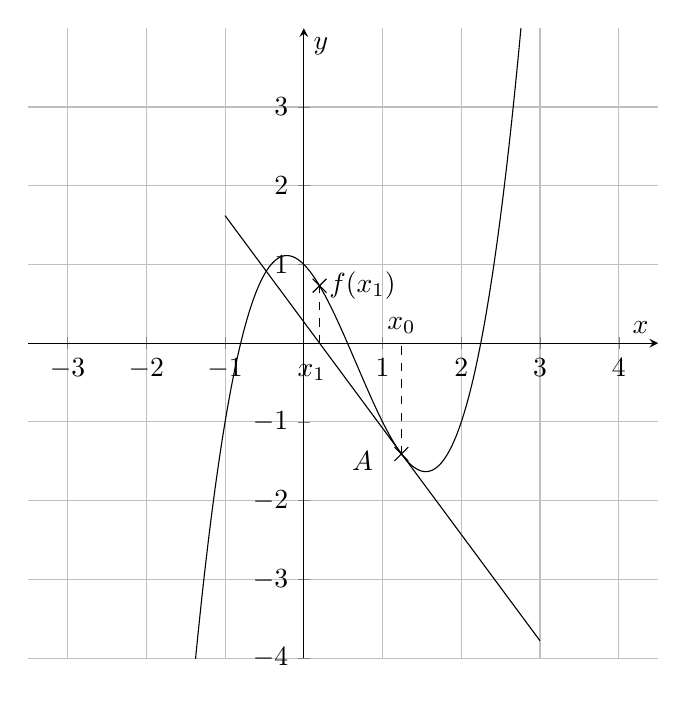
\begin{tikzpicture}
        \begin{axis}[xmin= -3.5, xmax = 4.5, ymin= -4, ymax= 4,
         x=1cm,y=1cm,
        axis lines = middle, 
        ymajorgrids=true,
        xmajorgrids=true,
        xtick={-3, -2, -1, 0, ..., 4},
        ytick={-4, -3, -2, ..., 3},
        xlabel = $x$,
        ylabel=$y$]
            \addplot[color= black, samples = 300, domain= -2:3]{x^3-2*x^2-x^1 +1};
            \addplot[color= black, samples = 300, domain= -1:3]{-1.35*x^1 +0.27};
            \draw[dashed] (1.24,-1.41)  -- (1.24,0) node(xline)[above] {$x_0$};
            \draw (1,-1.5)   node[left] {$A$};
            \draw (1.2390888331407657,-1.4073470487766349)-- ++(-2.5pt,-2.5pt) -- ++(5pt,5pt) ++(-5pt,0pt) -- ++(5pt,-5pt);
            \draw[dashed] (0.2,0.2) node(xline)[above] {};
            \draw (0.1,-0.6)   node [above] {$x_1$};
            \draw[dashed] (0.2,0)  -- (0.2,0.73) node(xline)[right] {$f(x_1)$};
            \draw (0.2,0.73)-- ++(-2.5pt,-2.5pt) -- ++(5pt,5pt) ++(-5pt,0pt) -- ++(5pt,-5pt);
        \end{axis}
    \end{tikzpicture}     
\end{center}
\end{bsp}
Die einzelnen Iterationsschritte sind hierbei nicht immer von einzeln durchzuführen. Mit den aktuell erlaubten Taschenrechnern ist es möglich, die sich wiederholenden Schritte immer wieder durchzuführen\footnote{Siehe Anleitung Taschenrechner für die Programmierung.}.
\end{section}
\section{Kurvendiskussion}
 \subsection{Monotonie und Extrema}   
 \begin{defi}{Monotonie}{}\index{Kurvendiskussion!Monotonie}\index{Monotonie}
 Es sei $f$ eine Funktion auf einem Intervall $I$ definiert. Gilt für alle $x_1, x_2 \in I$ mit $x_1<x_1:$
 \begin{equation*}
	\left.\begin{aligned}
	f(x_1) &<  f(x_2)  \\
	f(x_1) &> f(x_2)
	\end{aligned}
	\right\}
\quad \text{So nennt man f}
	\quad\left\{\begin{aligned}
	\text{monoton steigend}  \\
	\text{monoton fallend}
	\end{aligned}
\right\}
\quad
 \text{im Intervall I} 
\end{equation*} 
 \end{defi}
 \begin{defi}{Extrema}{}
   Es sei $f$ eine auf einem Intervall $I$ definierte Funktion. Dann nennt man $f(x_0)$ \textcolor{red}{lokales Maximum} wenn es eine Umgebung $U$ um $x_0$ gibt, sodass für alle  $x \in U \in \mathds{D_f}$ gilt: \textcolor{red}{$f(x_0)\geq f(x)$}. Der Punkt \textcolor{red}{$P(x_0|f(x_0))$} heißt dann \textcolor{red}{Hochpunkt (HoP)}.\\
   Es sei $f$ eine auf einem Intervall $I$ definierte Funktion. Dann nennt man $f(x_0)$ \textcolor{red}{lokales Minimum} wenn es eine Umgebung $U$ um $x_0$ gibt, sodass für alle  $x \in U \in \mathds{D_f}$ gilt: \textcolor{red}{$f(x_0)\leq f(x)$}. Der Punkt \textcolor{red}{$P(x_0|f(x_0))$} heißt dann \textcolor{red}{Tiefpunkt (TiP)}.
 \end{defi}
 \begin{satz}{Bedingung für die Monotonie}{}\index{Monotonie!Bedingung}
 Ist die Funktion $f$ im Intervall $I$ eine differenzierbare Funktion und 
  \begin{equation*}
	\left.\begin{aligned}
	f'(x) &>0  \\
	f'(x) &<0
	\end{aligned}
	\right\}
\quad \text{für alle $x\in I$, dann ist $f$ in $I$ streng monoton}
	\quad\left\{\begin{aligned}
	\text{wachsend}  \\
	\text{fallend}
	\end{aligned}
\right.
\end{equation*} 
 \end{satz}
 \begin{satz}{Notwendige Bedingung für innere Extrempunkt}{}\index{Monotonie!Notwendige Bedingung}
   Eine Funktion $f$ und ihre Ableitung $f'$ seien auf einem Intervall $I$ definiert. Dann gilt: \textcolor{red}{Hat} $f$ an einer inneren Stelle $x_0\in I$ einen \textcolor{red}{Extremwert}, so ist \textcolor{red}{$f'(x_0)=0$}
 \end{satz}
 \begin{b8d}{Vorzeichenwechsel und Extrema}{}\index{Monotonie!Vorzeichenwechsel}
 Die Art der einzelnen Extrema läßt sich leicht durch die Vorzeichenwechsel (VZW) der Ableitung bestimmen.
 \begin{itemize}
\item Hochpunkt (HoP) $HoP(x_0|f(x_0))$ genau dann, wenn es einen VZW der Ableitung von \textcolor{red}{positiv nach negativ} gibt
\begin{enumerate}
    \item $f'(x_0) = 0$
    \item $x_i<x_0 \Rightarrow f'(x_i)>0$
    \item $x_0 <x_i \Rightarrow f'(x_i)<0$
\end{enumerate}
\item Tiefpunkt (TiP) $TiP(x_0|f(x_0))$ genau dann, wenn es einen VZW der Ableitung von \textcolor{red}{negativ nach positiv} gibt
\begin{enumerate}
    \item $f'(x_0) = 0$
    \item $x_i<x_0 \Rightarrow f'(x_i)<0$
    \item $x_0 <x_i \Rightarrow f'(x_i)>0$
\end{enumerate}
\item Terrassenpunkt (TP) $TP(x_0|f(x_0))$
\begin{enumerate}
    \item $f'(x_0) = 0$
    \item \textcolor{red}{kein VZW}
\end{enumerate}
 \end{itemize}
 \end{b8d}
 \begin{bsp}{Bestimmung der Monotonie und der Extrema I}{}
 Gegeben ist die Funktion $f(x) = 2x^3 +6x^2 -2x + 1$ mit $\mathds{D}_f = \mathds{R}$ und der ersten Ableitung $f'(x) = 6x^2+12x-2$.\\
 Vorgehen:
 \begin{enumerate}
     \item Bestimmung der Nullstelle der ersten Ableitung
     \item Untersuchung der Monotonie mit Hilfe der Monotonietabelle
     \item Entscheidungen zu möglichen Extrema
 \end{enumerate}
 \begin{center}$\begin{aligned}
	f'(x)&= 6x^2+12x-2\\
    0 &= 6x^2+12x-2\\
    x_{1,2} &= \dfrac{-12 \pm \sqrt{144 +48} }{12} = \dfrac{-12\pm 8\sqrt{3}}{12}\\
    &= \dfrac{-3\pm 2\sqrt{3}}{3}\\
    x_1&= \dfrac{-3+ 2\sqrt{3}}{3}\\
    x_2&= \dfrac{-3 - 2\sqrt{3}}{3}
	\end{aligned}$\end{center}
 Mit diesen beiden Nullstellen ist es möglich eine faktorisierte Form des Funktionsterms aufzuschreiben. $$f'(x)= 6x^2+12x-2 = 6\cdot \left(x-x_1 \right)\cdot \left(x-x_2 \right)$$
Monotonietabelle:\\
\begin{center}\begin{tabular}{||c|c|c|c|c|c||}
    \hline
    $x$& $ -\infty <x<x_2 $ & $ x_2 \approx -2.15$ &$ x_2<x<x_1 $ & $x_1 \approx 0,15 $& $ x_1<x<\infty $\\
    \hline \hline
    $6\cdot (x-x_2)$ & + &  0 & - &  & +  \\
    \hline
    $(x -x_1)$ & - & & + &0 & + \\
    \hline
    $f'(x)$ & + & 0 & - & 0 & +\\ 
    \hline
    $G_f$ & smw & HoP & smf & TiP & smw\\
    \hline
\end{tabular}
\end{center}
\begin{center}
    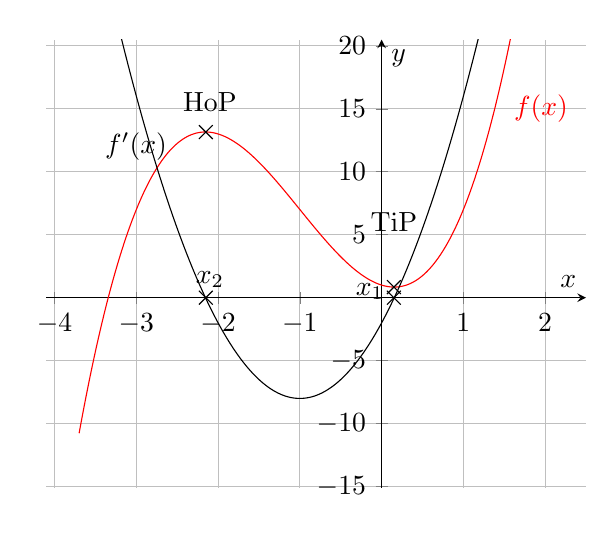
\begin{tikzpicture}
        \begin{axis}[xmin= -4.1, xmax = 2.5, ymin= -15.1, ymax= 20.5,
        axis lines = middle, 
        ymajorgrids=true,
        xmajorgrids=true,
        xtick={-4, -3,  ..., 2},
        ytick={-15, -10, -5, ..., 20},
        xlabel = $x$,
        ylabel=$y$]
            \addplot[color= red, samples = 300, domain= -3.7:1.7]{2*x^3+ 6*x^2 -2*x+1};
         \draw (1.5,15)   node [right] {\textcolor{red}{$f(x)$}};  
            \addplot[color= black, samples = 300, domain= -3.7:1.7]{6*x^2+ 12*x -2};
            \draw (-3.5,12)   node [right] {$f'(x)$}; 
            \draw (-2.1,0)   node [above] {$x_2$};
            \draw (0.15,0.5)   node [left] {$x_1$};
             \draw (-2.15,0)-- ++(-2.5pt,-2.5pt) -- ++(5pt,5pt) ++(-5pt,0pt) -- ++(5pt,-5pt);
             \draw (-2.1,14)   node [above] {HoP};
              \draw (-2.15,13.15)-- ++(-2.5pt,-2.5pt) -- ++(5pt,5pt) ++(-5pt,0pt) -- ++(5pt,-5pt);
               \draw (0.15,0.84)-- ++(-2.5pt,-2.5pt) -- ++(5pt,5pt) ++(-5pt,0pt) -- ++(5pt,-5pt);
               \draw (0.15,4.5)   node [above] {TiP};
              \draw (0.15,0)-- ++(-2.5pt,-2.5pt) -- ++(5pt,5pt) ++(-5pt,0pt) -- ++(5pt,-5pt);
        \end{axis}
    \end{tikzpicture}  
\end{center}
\end{bsp}
\begin{bsp}{Bestimmung der Monotonie und der Extrema II}{}
Betrachtet wird die Funktion $f(x)= x^3-6x^2 +9x-2$ mit $\mathds{D}_f =\mathds{R}$ und der ersten Ableitung $f'(x)= 3x^2 -12x +9$
\begin{center}$\begin{aligned}
	f'(x)&= 3x^2 -12x +9\\
    0 &= 3x^2 -12x +9\\
    x_{1,2} &= \dfrac{12 \pm \sqrt{144 -8} }{6} = \dfrac{12\pm \sqrt{36}}{6} = \dfrac{12 \pm 6}{6} = 2\pm 1\\
    x_1&= 3\\
    x_2&= 1
	\end{aligned}$\end{center}
 Mit diesen beiden Nullstellen ist es möglich eine faktorisierte Form des Funktionsterms aufzuschreiben. $$f'(x)= 3x^2-12x+9 = 3\cdot \left(x-3 \right)\cdot \left(x-1 \right)$$

Monotonietabelle:\\
\begin{center}\begin{tabular}{||c|c|c|c|c|c||}
    \hline
    $x$& $ -\infty <x<1 $ & $ x_2 =1$ &$ 1<x<3 $ & $x_1 = 3 $& $ 3<x<\infty $\\
    \hline \hline
    $3\cdot (x-1)$ & - &  0 & + &  & +  \\
    \hline
    $(x -3)$ & - & & - & 0 & + \\
    \hline
    $f'(x)$ & + & 0 & - & 0 & +\\ 
    \hline
    $G_f$ & smw & $HoP(1|2)$ & smf & $TiP(3|-2) $& smw\\
    \hline
\end{tabular}
\end{center}
\begin{center}
    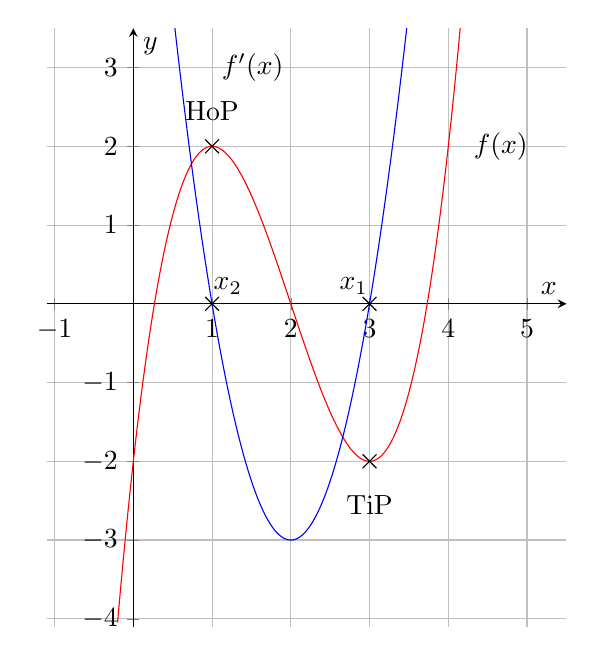
\begin{tikzpicture}
        \begin{axis}[xmin= -1.1, xmax = 5.5, ymin= -4.1, ymax=3.5,
         x=1cm,y=1cm,
        axis lines = middle, 
        ymajorgrids=true,
        xmajorgrids=true,
        xtick={-4, -3, -2,  ..., 5},
        ytick={-4, -3, -2, ..., 3},
        xlabel = $x$,
        ylabel=$y$]
            \addplot[color= red, samples = 300, domain= -0.2:4.2]{x^3-6*x^2+9*x-2};
     \addplot[color= blue, samples = 300, domain= -0.2:4.2]{3*x^2-12*x+9};
            \draw (4.2,2)   node [right] {$f(x)$}; 
            \draw (1,3)   node [right] {$f'(x)$}; 
            \draw (1.2,0)   node [above] {$x_2$};
            \draw (2.8,0)   node [above] {$x_1$};
             \draw (1,0)-- ++(-2.5pt,-2.5pt) -- ++(5pt,5pt) ++(-5pt,0pt) -- ++(5pt,-5pt);
              \draw (3,0)-- ++(-2.5pt,-2.5pt) -- ++(5pt,5pt) ++(-5pt,0pt) -- ++(5pt,-5pt);
               \draw (1,2.2)   node [above] {HoP};
                \draw (1,2)-- ++(-2.5pt,-2.5pt) -- ++(5pt,5pt) ++(-5pt,0pt) -- ++(5pt,-5pt);
                 \draw (3,-2)-- ++(-2.5pt,-2.5pt) -- ++(5pt,5pt) ++(-5pt,0pt) -- ++(5pt,-5pt);
               \draw (3,-2.8)   node [above] {TiP};
        \end{axis}
    \end{tikzpicture}  
\end{center}
\end{bsp}
\begin{bem}{Tangentengleichungen}{}
Eine klassische Aufgabe innerhalb der Kurvendiskussion bildet die Bestimmung einer Tangente an einen beliebigen Punkt des Graphen. Hierfür ist es notwendig folgende Informationen zu bestimmen:
\begin{enumerate}
    \item Bildung der ersten Ableitung
    \item Berechnung der Koordinaten des Punktes auf dem Graphen
    \item Bestimmung der Steigung des Graphen in diesem Punkt
    \item Aufstellen der Geradengleichung der Tangente
\end{enumerate}
\end{bem}
\label{Tangentengleichung}
\begin{bsp}{Bestimmung der Tangentengleichung}{}\index{Kurvendiskussion!Tangentengleichung}
  Betrachtet wird die Funktion $f(x)= x^3 -6x^2 +9x -2$ mit $\mathds{D}_f = \mathds{R}$ und der Punkt $P(2|0)$.
 \begin{center}$\begin{aligned}
	f'(x)&= 3x^2 -12x +9\\
    f'(2) &= 3\cdot 2^2 -12 \cdot 2 +9 = -3
	\end{aligned}$\end{center} 
 Aufstellen der Tangentengleichung aus den berechneten Werten $P(2|0)$ und $m= f'(2) = -3$: 

\begin{equation*}
	\left.\begin{aligned}
	0 &=  f'(2) \cdot 2 + t \\
	0 &= -3 \cdot 2 +t\\
    t &=6
	\end{aligned}
	\right\}
\quad \text{damit folgt für die Tangentengleichung:}\hspace{0.1cm } y_T = -3\cdot x +6 
\end{equation*}
\end{bsp}
\subsection{Die Extremstellen der lokalen Änderungsrate - Wendestellen} \index{Krümmungsverhalten} \index{Kurvendiskussion!Krümmungsverhalten}
\begin{defi}{Der Wendepunkt}{}\index{Krümmungsverhalten!Wendepunkt}\index{Kurvendiskussion!Wendepunkt}
Der Punkt, an dem sich die Krümmung des Graphen der Funktion $f$ ändert, heißt Wendepunkt. Am Wendepunkt des Graphen liegt ein Extremwert der lokalen Änderungsrate vor. Ein Terrassenpunkt ist ein Wendepunkt mit einer waagerechten Tangente.
\end{defi}

\begin{satz}{Zusammenhang der lokalen Änderungsrate und der Krümmung}{krümmung}
  Wenn die lokale Änderungsrate $f'$ einer differenzierbaren Funktion $f$ im Intervall $I$ \textcolor{red}{streng monoton zunimmt}, dann ist der Graph $G_f$ \textcolor{red}{linksgekrümmt}.  \\
  Wenn die lokale Änderungsrate $f'$ einer differenzierbaren Funktion $f$ im Intervall $I$ \textcolor{red}{streng monoton abnimmt}, dann ist der Graph $G_f$ \textcolor{red}{rechtsgekrümmt}. 
\end{satz}
\begin{satz}{Kriterium der Krümmung}{}
Ist die Funktion $f$ im Intervall $I$ zweimal stetig differenzierbar und ist für alle $a\in I$ der Funktionswert $f''(x)$ \textcolor{red}{positiv}, dann ist der Graph der Funktion $f$ \textcolor{red}{linksgekrümmt}.\\
Ist die Funktion $f$ im Intervall $I$ zweimal stetig differenzierbar und ist für alle $a\in I$ der Funktionswert $f''(x)$ \textcolor{red}{negativ}, dann ist der Graph der Funktion $f$ \textcolor{red}{rechtsgekrümmt}.

\index{Krümmungsverhalten!Kriterium}\end{satz}
\begin{bem}{Extremwert der Änderungsrate}{}
Der Punkt, an dem sich die Krümmung des Graphen ändert, heißt \textcolor{red}{Wendepunkt}. Beim \textcolor{red}{Wendepunkt} liegt ein \textcolor{red}{Extremwert} der lokalen Änderungsrate vor. Ein \textcolor{red}{Terrassenpunkt} ist ein \textcolor{red}{Wendepunkt mit einer waagerechten Tangente}.
\end{bem}
Die Krümmung wird, genau wie Monotonieuntersuchung, durch eine Vorzeichentabelle untersucht.  
\begin{bsp}{Untersuchung der Krümmung}{}
Untersucht wird die Krümmung des Graphen der Funktion $f(x) = x^3 -3x^2$ mit $\mathds{D}_f = \mathds{R}$. Bestimmung der ersten und zweiten Ableitung der Funktion f.
\begin{equation*}
    \begin{split}
        f(x) &= x^3 -3x^2\\
        f'(x) &= 3x^2 -6x\\
        f''(x) &= 6x -6 = 6\cdot(x-1)
    \end{split}
\end{equation*}
Berechnung der Nullstelle der zweiten Ableitung:
\begin{equation*}
    \begin{split}
        0 &= 6\cdot(x-1) \hspace{0.2cm} | : 6\\
        0 &= x-1\hspace{0.9cm} | + 1\\
        x &= 1 
    \end{split}
\end{equation*}
\begin{center}\begin{tabular}{||c|c|c|c||}
    \hline
    $x$& $ -\infty <x<1$ & $x = 1$ & $ 1<x<\infty$ \\
    \hline \hline
    $f''(x)=6(x-1)$ & - & 0 & +\\
    \hline
    $G_f$ & rechtsgekrümmt & Wendepunkt $WP(1|-2)$ & linksgekrümmt\\
    \hline
    \hline
\end{tabular}
\end{center}
Berechnung der Koordinaten des Wendepunktes:
\begin{equation*}
    \begin{split}
        f(1) &= (1)^3 -3\cdot (1)^2\\
         &= 1 - 3 \\
         &= -2 
    \end{split}
\end{equation*}
\begin{center}
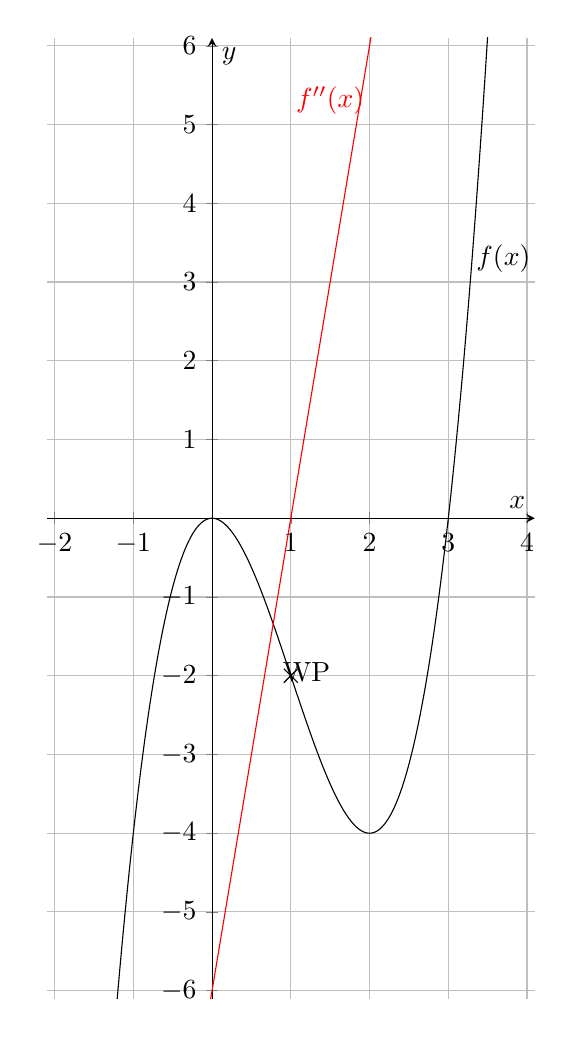
\begin{tikzpicture}
    \begin{axis}[xmin= -2.1, xmax = 4.1, ymin= -6.1, ymax=6.1,
     x=1cm,y=1cm,
        axis lines = middle, 
        ymajorgrids=true,
        xmajorgrids=true,
        xtick={-2, -1, -0,  ..., 4},
        ytick={-6, -5, -4, ..., 6},
        xlabel = $x$,
        ylabel=$y$]
        \addplot[color= black, samples = 300, domain= -1.8:3.8]{x^3 -3*x^2};
        \addplot[color= red, samples = 300, domain= -1.8:3.8]{6*x -6};
        \draw (1,-2)-- ++(-2.5pt,-2.5pt) -- ++(5pt,5pt) ++(-5pt,0pt) -- ++(5pt,-5pt);
        \draw (1.2,-2.2)   node [above] {WP};
        \draw[red] (1.5,5)   node [above] {$f''(x)$};
        \draw (3.7,3)   node [above] {$f(x)$};

    \end{axis}
\end{tikzpicture}
\end{center}
\end{bsp}
\begin{b8d}{}{}
Ein Wendepunkt liegt nur vor, wenn sich das Krümmungsverhalten ändert.
\end{b8d}
\subsection{Ausführliche Untersuchung ganzrationaler Funktionen} \index{Kurvendiskussion!Vollständige Untersuchung }
Die ausführliche Kurvendiskussion besteht aus einer Reihe von analytischen Untersuchungen des Terms der Funktion um damit auf das Verhalten des Graphen der Funktion zu schließen. Hierbei ist es allerdings nicht notwendig alle Schritte auswendig zu lernen.
\begin{merke}{Schritte der ausführlichen Kurvendiskussion}{}
\begin{enumerate}
    \item Untersuchungen am ursprünglichen Term
    \begin{itemize}
        \item Bestimmung des maximalen Definitionsbereichs
        \item Untersuchungen der Symmetrie
        \item Verhalten an den Rändern des Definitionsbereichs 
        \item Gemeinsame Punkte mit den Koordinatenachsen
    \end{itemize}
    \item Untersuchungen des Terms der ersten Ableitung
        \begin{itemize}
            \item Monotonie
            \item Extrempunkte

        \end{itemize}
    \item Untersuchungen des Terms der zweiten Ableitung
        \begin{itemize}
            \item Krümmungsverhalten
            \item Tangentensteigungen von speziellen Punkten
        \end{itemize}
    \item Graph der Funktion mit allen berechneten Werten
    \item Wertemenge der Funktion
\end{enumerate}
\end{merke}

\begin{bsp}{Ausführliche Kurvendiskussion}{}
Betrachtet wird die Funktion $f(x)= \dfrac{1}{16} x^4 +\dfrac{1}{4} x^3$ mit $\mathds{D}_f =\mathds{D}_{max}$ dem maximalen Definitionsbereich. Es soll für die Funktion eine vollständige Kurvendiskussion durchgeführt werden.
\begin{enumerate}
    \item Bestimmung des maximalen Definitionsbereichs: $\mathds{D}_f = \mathds{R}$
    \item Untersuchungen der Symmetrie:
    $$f(-x) = \frac{1}{16} \cdot (-x)^4 + \frac{1}{4} \cdot (-x)^3 = \frac{1}{16} \cdot x^4 - \frac{1}{4} \cdot x^3 \neq \pm f(x)$$ Damit ist der Graph $G_f$ weder punktsymmetrisch zum Ursprung noch achsensymmetrisch zur y-Achse.
    \item Verhalten an den Rändern des Definitionsbereichs
    $$\lim_{x\rightarrow \infty} f(x) = \lim_{x\rightarrow \infty} \dfrac{1}{16}x^4 +\dfrac{1}{4}x^3 = \infty$$
        $$\lim_{x\rightarrow -\infty} f(x) = \lim_{x\rightarrow -\infty} \dfrac{1}{16}x^4 +\dfrac{1}{4}x^3 = \infty$$
        Das Verhalten von Polynomen an den Rändern des Definitionsbereichs wird durch den Summanden mit der höchsten Potenz (Grad des Polynoms) festgelegt. In diesem Beispiel ist der Grad $n=4$ und damit streben die Funktionswerte an den Rändern des Definitionsbereichs gegen Unendlich.
    \item Gemeinsame Punkte mit den Koordinatenachsen:
    \begin{itemize}
        \item Schnittpunkt mit der y-Achse
    
    \begin{equation*}
        f(0) = \dfrac{1}{16}0^4 +\dfrac{1}{4}0^3 = 0
    \end{equation*}
    Damit liegt der Schnittpunkt mit der y-Achse bei $SP_y(0|0)$.
    \item Schnittpunkte mit der x-Achse
    \begin{equation*}
        \begin{split}
         0 &= \dfrac{1}{16} x^3 (x+4)\\
             x_1 =x_2=x_3&= 0 \longrightarrow SP_{x_1} = SP_{x_2} = SP_{x_3}(0|0) \\
             x_4&= -4 \longrightarrow SP_{x_4}(-4|0)
        \end{split}
\end{equation*}
    \end{itemize}
  \item Monotonie des Graphen $G_f$ der Funktion $f$:  
    \begin{itemize}
        \item Bildung der Ableitungen
    \begin{equation*}
        \begin{split}
        f(x) &= \dfrac{1}{16} x^4 +\dfrac{1}{4} x^3\\
            f'(x)&= \dfrac{1}{4} x^3 +\dfrac{3}{4} x^2\\
            f''(x) &= \dfrac{3}{4} x^2 + \dfrac{3}{2} x
        \end{split}
\end{equation*}
       \item Berechnung der Nullstellen der ersten Ableitung 
           \begin{equation*}
        \begin{split}
         0 &= \dfrac{1}{4} x^3 +\dfrac{3}{4} x^2\\
         0 &= \dfrac{1}{4} x^2 (x+3)\\
         x_1 =x_2 &= 0\\
         x_3&= -3
        \end{split}
\end{equation*}

Monotonietabelle:
\begin{center}\begin{tabular}{||c|c|c|c|c|c||}
    \hline
    $x$& $ -\infty <x<-3 $ & $ x = -3$ &$ -3<x<0 $ & $x=0 $& $ 0<x<\infty $\\
    \hline \hline
    $\frac{1}{4} x^2$ & + &  0 & + &  & +  \\
    \hline
    $(x +3)$ & - & 0 & + &  & + \\
    \hline

    $f'(x)$ & - & 0 & + & 0 & +\\ 
    \hline
    \hline
    $G_f$ & smf & $TiP(-3|-\frac{27}{16})$ & smw  & $TP(0|0) $& smw\\
    \hline
\end{tabular}
\end{center}
Berechnung der Koordinaten:
           \begin{equation*}
        \begin{split}
         f(-3)&= \dfrac{1}{16} (-3)^4 +\dfrac{1}{4} (-3)^3\\
         &= -\dfrac{27}{16}\approx -1,69\\
         f(0) &= \dfrac{1}{16} 0^4 +\dfrac{1}{4} 0^3 = 0
        \end{split}
\end{equation*}
Durch die Monotonietabelle ist es möglich, dass gleichzeitig die Art der Extrempunkte bestimmt werden kann.
    \end{itemize}
    \item Bestimmung des Krümmungsverhalten:
 \begin{equation*}
        \begin{split}
         0 &= \dfrac{3}{4} x^2 +\dfrac{3}{2} x\\
         0 &= \dfrac{3}{2} x \cdot (\dfrac{1}{2}x + 1)\\
         x_1 &= 0\\
         x_2&= -2
        \end{split}
\end{equation*}
Krümmungstabelle:
\begin{center}\begin{tabular}{||c|c|c|c|c|c||}
    \hline
    $x$ & $ -\infty <x<-2 $ & $ x = -2$ &$ -2<x<0 $ & $x=0 $& $ 0<x<\infty $\\
    \hline \hline
    $\frac{3}{2} x$ & - &  -3 & - & 0 & +  \\
    \hline
    $(\frac{1}{2} x +1)$ & - & 0 & + & 1 & + \\
    \hline

    $f''(x)$ & + & 0 & - & 0 & +\\ 
    \hline
    \hline
    $G_f$ & linksgekrümmt & $TP(-2|-1)$ & rechtsgekrümmt  & $TP(0|0) $& linksgekrümmt\\
    \hline
\end{tabular}
\end{center}
Berechnung der Koordinaten:
           \begin{equation*}
        \begin{split}
         f(-2)&= \dfrac{1}{16} (-2)^4 +\dfrac{1}{4} (-2)^3\\
         &= 1-2 \\
         &= -1\\
         f(0) &= \dfrac{1}{16} 0^4 +\dfrac{1}{4} 0^3 = 0
        \end{split}
\end{equation*}
\item Berechnung der Wendetangente am Terrassenpunkt $TP(-2|-1)$:
\begin{itemize}
    \item Berechnung der Steigung des Graphen im Punkt $TP(-2|-1)$ 
    \begin{equation*}
        \begin{split}
         f'(-2)&= \dfrac{1}{4} (-2)^3 +\dfrac{3}{4} (-2)^2\\
         &= -2+3\\
         &= 1
        \end{split}
\end{equation*}
\item Berechnung des y-Achsenabschnitts
\begin{equation*}
        \begin{split}
        y &= m \cdot x +t \\
         -1 &= 1\cdot -2 +t \\
        -1 &= -2 +t \\
        t &= 1\\
         y&= 1\cdot x +1
        \end{split}
\end{equation*}
\end{itemize}
\item Wertemenge: $\mathds{W}= [-\dfrac{27}{16} \hspace{0.1cm}|\hspace{0.1cm} \infty \hspace{0.1cm}[ $
\item Graph der Funktion:
\begin{center}
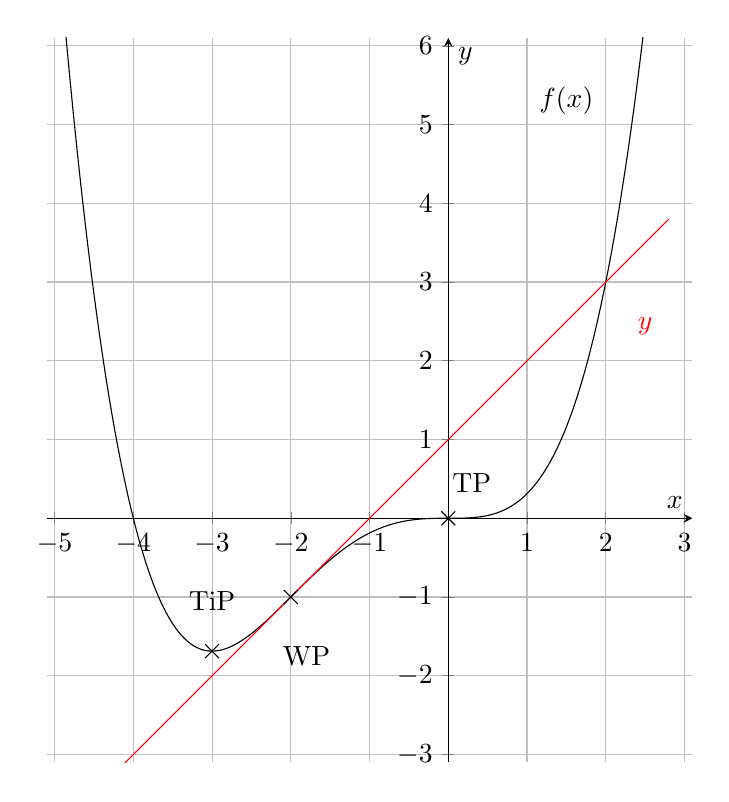
\begin{tikzpicture}
    \begin{axis}[xmin= -5.1, xmax = 3.1, ymin= -3.1, ymax=6.1,
     x=1cm,y=1cm,
        axis lines = middle, 
        ymajorgrids=true,
        xmajorgrids=true,
        xtick={-5, -4, -3,  ..., 3},
        ytick={-3, -2, ..., 6},
        xlabel = $x$,
        ylabel=$y$]
        \addplot[color= black, samples = 300, domain= -5:2.8]{1/16 * x^4 + 1/4*x^3};
        \addplot[color= red, samples = 300, domain= -4.8:2.8]{x +1};
        \draw (-3,-27/16) -- ++(-2.5pt,-2.5pt) -- ++(5pt,5pt) ++(-5pt,0pt) -- ++(5pt,-5pt);
        \draw (-3,-1.3)   node [above] {TiP};
        \draw (0,0) -- ++(-2.5pt,-2.5pt) -- ++(5pt,5pt) ++(-5pt,0pt) -- ++(5pt,-5pt);
         \draw (0.3,0.2)   node [above] {TP};
        \draw (-2,-1) -- ++(-2.5pt,-2.5pt) -- ++(5pt,5pt) ++(-5pt,0pt) -- ++(5pt,-5pt);
         \draw (-1.8,-2)   node [above] {WP};
        \draw (1.5,5)   node [above] {$f(x)$};
        \draw[red] (2.5,2.2)   node [above] {$y$};

    \end{axis}
\end{tikzpicture}
\end{center}
\end{enumerate} 
\end{bsp}
\section{Die Stammfunktion}\index{Stammfunktion}
\begin{defi}{Die Stammfunktion}{}
    Unter einer Stammfunktion einer Funktion $f$ versteht man die differenzierbare Funktion $F$, deren Ableitungsfunktion $F'$ mit $f$ übereinstimmt. Ist also $f$ auf einem Intervall $I$ definiert, so muss auch $F$ auf $I$ definiert und differenzierbar sein. Damit muss für alle $x\in I$ gelten: $$F'(x)= f(x).$$
\end{defi}
\begin{satz}{Stammfunktion der Potenzfunktion}{}\index{Stammfunktion!Potenzfunktion}
    Die Potenzfunktion $f: x \longrightarrow x^n$  mit $\mathds{D}_f = \mathds{R}$ ist auf ganz $\mathds{R}$ stetig. Die Menge aller Stammfunktion der Potenzfunktion lautet damit: $$F(x)= \dfrac{1}{n+1} \cdot x^{n+1} + c .$$
    Die additive Konstante c mit $c\in\mathds{R}$ steht hierbei die absoluten Anteil der Potenzfunktion.
\end{satz}
\begin{b8d}{Die Menge der Stammfunktionen}{}\index{Stammfunktion!Menge aller Stammfunktionen}
Durch die additive Konstante $c$ wird die Menge der Stammfunktionen beschrieben. Sollen also {\bfseries\textcolor{red}{alle}} Stammfunktionen angegeben werden, muss die Konstante $c$ stehts mit angegeben werden. Wird nur eine Stammfunktion verlangt, reicht es, dass nur ein Wert für $c$ eingesetzt wird.
\end{b8d}
\begin{bsp}{Beispiele der Stammfunktion}{}
Für alle Konstanten $c$ gilt $c\in \mathds{R}$.
\begin{itemize}
    \item $f(x) = x^4 \hspace{0.2cm} \longrightarrow \hspace{0.2cm} F(x) = \dfrac{1}{5}\cdot x^5 + c $
    \item $f(x) = -\dfrac{3}{4}\cdot x^7 \hspace{0.2cm} \longrightarrow \hspace{0.2cm} F(x)= -\dfrac{3}{4} \cdot \dfrac{1}{8} \cdot x^8 + c$
    \item $f(x)= 3\cdot x^4 + 2 \hspace{0.2cm} \longrightarrow \hspace{0.2cm} F(x) = 3\cdot \dfrac{1}{5}\cdot x^5 + 2\cdot x + c$
    \item $f(x) = x^2 +a^2 \hspace{0.2cm} \longrightarrow \hspace{0.2cm} F(x)= \dfrac{1}{3} \cdot x^3 + a^2 \cdot x + c$
\end{itemize}
\end{bsp}
\section{Funktionenscharen}\index{Funktionen!Funktionenscharen}
Unter Funktionsscharen versteht man Funktion, die neben der \glqq normalen\grqq{} Variablen $x$ noch einen oder mehrere Parameter besitzen. Diese Parameter werden in der Kurvendiskussion als Zahlen interpretiert. 
\begin{defi}{Definition von Funktionenscharen}{}
Bei einer Funktionenschar gibt es neben der Variable $x$ auch noch einen Parameter (häufig a oderk), welchen man frei auf eine Zahl festlegen kann. Für jede Besetzung des Parameters bekommt man einen anderen Funktionsterm und somit auch einen anderen Funktionsgraphen.
\end{defi}
\begin{bsp}{Beispiel für einen Funktionenschar}{}
Betrachtet wird die Funktionenschar $f_a(x) = x^2 +a$ mit $\mathds{D}_{f_a} = \mathds{R}$ und $a \in \mathds{R}$. Wie man leicht sieht, realisiert der Parameter $a$ eine Verschiebung des Graphen von $f_a(x)$ entlang der $y-Achse$. So gilt für $a>0$, dass der Graph $G_{f_a}$ nach oben und für $a<0$ nach unten verschoben wird. Für den Wert $a= 0$ erhält man die Normalparabel.
\begin{center}
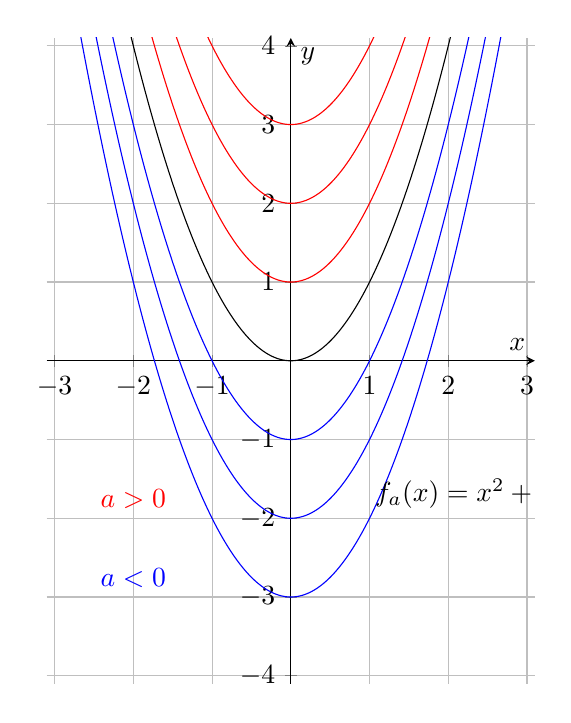
\begin{tikzpicture}
    \begin{axis}[xmin= -3.1, xmax = 3.1, ymin= -4.1, ymax=4.1,
     x=1cm,y=1cm,
        axis lines = middle, 
        ymajorgrids=true,
        xmajorgrids=true,
        xtick={-3, -2, -1,  ..., 3},
        ytick={-4, -3, ..., 4},
        xlabel = $x$,
        ylabel=$y$]
        \addplot[color= red, samples = 300, domain= -2.8:2.8]{x^2 +3};
        \addplot[color= red, samples = 300, domain= -2.8:2.8]{x^2 +2};
        \addplot[color= red, samples = 300, domain= -2.8:2.8]{x^2 +1};
        \addplot[color= black, samples = 300, domain= -2.8:2.8]{x^2};
        \addplot[color= blue, samples = 300, domain= -2.8:2.8]{x^2 -1};
        \addplot[color= blue, samples = 300, domain= -2.8:2.8]{x^2 -2};
        \addplot[color= blue, samples = 300, domain= -2.8:2.8]{x^2 -3};
        \draw (1.5,5)   node [above] {$f(x)$};
        \draw (2.2,-2)   node [above] {$f_a(x) = x^2+a$};
        \draw[red] (-2,-2)   node [above] {$a>0$};
        \draw[blue] (-2,-3)   node [above] {$a<0$};
    \end{axis}
\end{tikzpicture}
\end{center}
\end{bsp}
\begin{bsp}{Kurvendiskussion von Funktionenscharen}{}
Betrachtet wird die Funktionenschar $f_a(x) = \dfrac{1}{8} \cdot (x^3 - 3a\cdot x +3a^2 \cdot x -12x)$ mit $\mathds{D}_{f_a} = \mathds{R}$ und $a \in \mathds{R}$. Der Graph $G_{f_a}$ soll jetzt in Abhängigkeit von $a$ auf Nullstellen und Extrema untersucht werden.
\begin{itemize}
    \item Bestimmung der Nullstellen:
\begin{equation*}
    \begin{split}
         0 &= \dfrac{1}{8} \cdot (x^3 - 3a\cdot x +3a^2 \cdot x -12x) \hspace{0.5cm} | \cdot 8\\
         0 &= x^3 - 3a\cdot x +3a^2 \cdot x -12x\\
         0 &= x\cdot(x^2 -3a + 3a^2 -12)\\
         x_1&= 0\\
         0 &= x^2 -3a+3a^2 -12\hspace{0.5cm} | +3a-3a^2+12\\
         x^2 &= 3a-3a^2+12\\
         x_{1/2} &= \pm \sqrt{3a-3a^2+12}
        \end{split}
\end{equation*}
An dieser Stelle muss eine Fallunterscheidung erfolgen. Hierbei wird untersucht, für welche Werte von $a$ der Wurzelterm keine, eine bzw. 2 Lösungen besitzt.
\begin{enumerate}
    \item Eine Lösung genau dann wenn die Diskriminante  Null ist. Das bedeutet:
    \begin{equation*}
    \begin{split}
         0 &= 3a-3a^2+12\\
       0 &= -3a^2 +3a +12 \\
       a_{1/2} &= \dfrac{-3 \pm \sqrt{3^2 -4\cdot (-3)\cdot 12}}{2\cdot (-3)}\\
       &= \dfrac{-3\pm \sqrt{9+144}}{-6}\\
       &= \dfrac{-3\pm 3\sqrt{17}}{-6}\\
       &= \dfrac{-1\pm \sqrt{17}}{-2}\\
       a_1&= \dfrac{-1 +\sqrt{17}}{-2}\approx -1,56\\
       a_2&= \dfrac{-1 -\sqrt{17}}{-2} \approx 2,56
        \end{split}
\end{equation*}
Daraus folgt, dass $G_{f_a}$ genau eine Nullstelle bei $x=0 $ hat, wenn der Parameter $a$ den Werte $a_1 = \dfrac{-1 +\sqrt{17}}{-2}$ bzw. $a_2=\dfrac{-1 -\sqrt{17}}{-2}$ annimmt.
\item Zwei Lösungen genau dann wenn der Parameter folgende Ungleichung erfüllt: $a_1 < a <a_2$. Daraus folgt, dass der $G_{f_a}$ genau drei Nullstellen besitzt.
\item Keine Lösung genau dann wenn folgende Beziehungen erfüllt sind $a< a_1$ und $a>a_2$. Das führt dazu, dass der Graph $G_{f_a}$ genau eine Nullstelle bei $x= 0$ hat.
\end{enumerate}
\item Bestimmung möglicher Extrema:
    \begin{equation*}
    \begin{split}
        f'(x) &= \dfrac{1}{8} \cdot (3x^2 -3a +3a^2 -12) = \dfrac{3}{8}\cdot (x^2-a+a^2-4)\\
        0 &= \dfrac{3}{8}\cdot (x^2-a+a^2-4) \hspace{0.5cm} |\cdot \dfrac{8}{3}\\
        0&= x^2-a+a^2-4 \hspace{0.5cm} | +a -a^2+4\\
        x^2&= -a^2+a+4\\ 
        x_{1/2} &= \pm \sqrt{-a^2+a+4}
        \end{split}
\end{equation*}
An dieser Stelle muss, wie bei der Bestimmung der Nullstellen, eine Fallunterscheidung erfolgen. Hierbei wird untersucht, für welche Werte von $a$ der Wurzelterm keine, eine bzw. 2 Lösungen besitzt.
\begin{enumerate}
    \item Eine Lösung genau dann wenn die Diskriminante Null ist. Das bedeutet:
        \begin{equation*}
    \begin{split}
        0 &= -a^2 +a +4\\
        a_{1/2} &= \dfrac{-1 \pm \sqrt{(-1)^2 - 4\cdot (-1) \cdot 4}}{2\cdot (-1)} = \dfrac{-1\pm \sqrt{1+16}}{-2}\\
        &= \dfrac{-1\pm \sqrt{17}}{-2}\\
        a_1&= \dfrac{-1 +\sqrt{17}}{-2}\approx -1,56\\
       a_2&= \dfrac{-1 -\sqrt{17}}{-2} \approx 2,56      
       \end{split}
\end{equation*}
Damit hat $f'_a(x)$ genau eine Nullstelle wenn der Parameter $a$ den Wert  $a= a_1$ bzw. $a = a_2$ annimmt.
\item Zwei Lösungen genau dann wenn der Parameter folgende Ungleichung erfüllt: $a_1<a<a_2$. Damit hat $f_a(x)$ genau zwei Nullsten.
\item Keine Lösung genau dann wenn folgende Beziehungen erfüllt sind $a<a_1$ bzw. $a>a_2$. Das führt dazu, dass $f'_a(x)$ keine Nullstellen besitzt.
    \end{enumerate}
Die Art der Extrema kann jetzt durch eine Vorzeichentabelle der ersten Ableitung oder das einsetzen der Werte $a_1$ bzw. $a_2$ in die zweite Ableitung herausgefunden werden. 
\end{itemize}
Im folgenden ist der Graph $G_{f_1}$ der Funktion $f_1(x) = \dfrac{1}{8}\cdot(x^3-12x)$ und $G_{f_{-2}}$  der Funktion $f_{-2}(x)= \dfrac{1}{8} \cdot(x^3 -6x+12x-12x) = \dfrac{1}{8}\cdot(x^3+6x)$ abgebildet.
\begin{center}
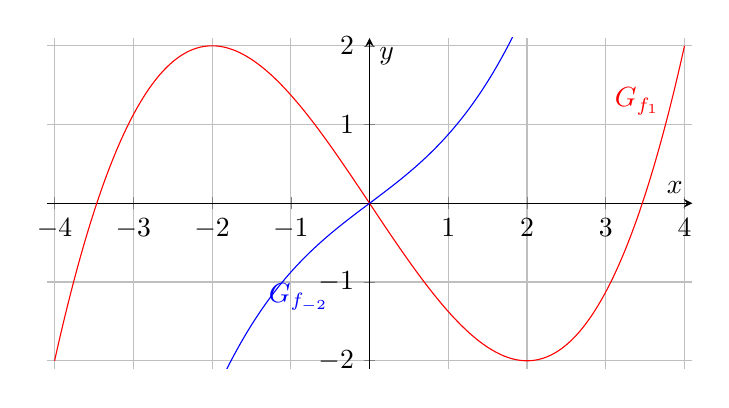
\begin{tikzpicture}
    \begin{axis}[xmin= -4.1, xmax = 4.1, ymin= -2.1, ymax=2.1,
     x=1cm,y=1cm,
        axis lines = middle, 
        ymajorgrids=true,
        xmajorgrids=true,
        xtick={-4, -3, -2,  ..., 4},
        ytick={-2, -1, ..., 2},
        xlabel = $x$,
        ylabel=$y$]
        \addplot[color= red, samples = 300, domain= -4:4]{1/8 * (x^3 -12*x)};
        \addplot[color= blue, samples = 300, domain= -4:4]{1/8 * (x^3 +6*x +12*x -12*x)};
        \draw[red] (3.4,1)   node [above] {$G_{f_1}$};
        \draw[blue] (-0.9,-1.5)   node [above] {$G_{f_{-2}}$};
    \end{axis}
\end{tikzpicture}
\end{center}
\end{bsp}
\section{Untersuchung von speziellen Funktionen}
    \subsection{Gebrochen-rationale Funktionen}
In der Jahrgangsstufe 8 erfolgten die einführenden Betrachtungen zu Elementaren gebrochen-rationalen Funktionen. Siehe hierzu im Anhang \ref{elemgebrat}.
 \begin{defi}{Gebrochen-rationale Funktion}{}
Eine Funktion $f$ mit $x\longrightarrow \dfrac{z(x)}{n(x)}$ nennt man gebrochen-rationale Funktion genau dann, wenn die Funktionen $z(x)$ und $n(x)$ Polynome sind. Die Funktion $f$ lässt sich damit durch folgenden Term beschreiben:$$f(x) = \dfrac{a_mx^m + a_{m-1}x^{m-1} + \ldots + a_1 x +a_0}{b_n x^n + b_{n-1}x^{n-1} + \ldots + b_1 x + b_0}$$ mit $m,n \in \mathds{R}$ und $a_m , b_n \neq 0$.
 \end{defi}
 \begin{bsp}{Beispiel für eine gebrochen-rationale Funktion}{} 
Der Graph der gebrochen-rationale Funktion  $$f(x)= \dfrac{x^2+4x+3}{x^2+x-2}$$ mit $\mathds{D}_f = \mathds{R}\setminus \{-2;1\}$. Aus der Hyperbel und den Definitionslücken kann man die beiden senkrechten Asymptoten bei $x=-2$ und bei $x=1$ ablesen.  
\begin{center}
\begin{tikzpicture}
    \begin{axis}[domain=-6:5, restrict y to domain=-5:5,axis x line=center, axis y line=center,%
     x=1cm,y=1cm,
xtick={-6,...,5}, ytick={-5,...,5}]
        \addplot[mark=none, color=red]  plot[samples=300,smooth]{((x+1)*(x+3)) / (x^2 +x - 2)};
        \draw[red] (3.4,1)   node [above] {$G_{f}$};

    \end{axis}
\end{tikzpicture}
\end{center}
\end{bsp}
 \begin{merke}{Eigenschaften gebrochen-rationaler Funktionen}{}
     \begin{enumerate}
         \item Die Nullstellen einer gebrochen-rationalen Funktion ergeben sich aus den Nullstellen des Zählerpolynoms.
         \item Die Stellen an den die Funktion nicht definiert ist ergeben sich aus den Nullstellen des Nennerpolynoms. Diese Nullstellen bilden die Definitionslücken. Damit ändert sich der Definitionsbereich der Funktion $f(x)= \dfrac{z(x)}{n(x)}$  für alle $x_i$ mit $n(x_i) = 0$ und $x_i \in \mathds{R}$ zu $\mathds{D}_f = \mathds{R}\setminus \left\{x_i\right\}$. 
     \item Eine gebrochen-rationale Funktion hat mehrere Darstellungsformen. Die oben bereits kennengelernte Bruchform und die sogenannte Summenform. Die Summenform setzt sich dabei aus einem Polynom und einem gebrochen-rationalen Term zusammen.
     \end{enumerate}
 \end{merke}
 In der Oberstufe werden gebrochen-rationale Funktionen meistens sowohl in der Bruch- als auch in der Summenform gegeben. Eine der typischen Aufgaben besteht dann darin, dass man die Äquivalenz der beiden Formen nachweist. Für die Polynomdivision siehe Anhang \ref{polynomdivision}  
 \begin{bsp}{Umwandlung der Formen einer gebrochen-rationalen Funktion}{}
Gegeben ist die Funktion $f$ mit $f(x) = \dfrac{x^3}{x^2-1} = x+ \dfrac{x}{x^2-1}$ und $\mathds{D}_f = \mathds{R}\setminus\{-1; 1\}$. Im folgenden soll die Äquivalenz der beiden Formen gezeigt werden.
\begin{enumerate}
    \item Von der Bruchform in die Summenform durch eine Polynomdivision:\\ \polylongdiv{x^3}{x^2-1}
    \item Durch erweitern der Summenform in die Bruchform: 
\begin{equation*}
    \begin{split}
        f(x) &= x+\dfrac{x}{x^2-1} \hspace{0.5cm} |\hspace{0.25cm} \text{erweitern mit } \hspace{0.25cm} (x^2-1)\\
        &= \dfrac{x\cdot (x^2-1)}{x^2-1} + \dfrac{x}{x^2-1}\\
        &= \dfrac{x^3-x}{x^2-1} + \dfrac{x}{x^2-1}\\
        &= \dfrac{x^3-x+x}{x^2-1} \\
        &= \dfrac{x^3}{x^2-1} = f(x)
    \end{split}
\end{equation*}
\end{enumerate}
\end{bsp}
 Beispielhaft soll im folgenden die Kurvendiskussion einer gebrochen-rationalen Funktion durchgeführt werden. 
 \begin{bsp}{Kurvendiskussion}{}\index{Funktionen!Gebrochen-rationale!Kurvendiskussion}
Gegeben ist die Funktion $f$ mit $f(x) = \dfrac{x^3-6x^2+9x}{(x-1)^2} = x-4+\dfrac{4}{(x-1)^2}$ mit $\mathds{D}_f = \mathds{D}_{\text{max}}$ dem maximalen Definitionsbereich. 
 \begin{enumerate}
     \item Der maximaler Definitionsbereich ergibt sich aus den Nullstellen des Nennerpolynoms\\ $(x-1)^2$
     \begin{equation*}
    \begin{split}
        n(x) &= (x-1)^2 \\
        0&= (x-1)^2\\
        x_{1} &= 1    
    \end{split}
\end{equation*}
Damit folgt für $\mathds{D}_{\text{max}}$ folgender Zusammenhang $\mathds{D}_{\text{max}} = \mathds{R}\setminus\{1\}$.
\item Symmetrie
\begin{equation*}
    \begin{split}
        f(-x) &= \dfrac{(-x)^3-6(-x)^2+9(-x)}{((-x)-1)^2} \\
        &= \dfrac{-x^3-6x^2-9x}{-x-1)^2}\\
         &\neq  f(x)\\
         &\neq -f(x)
    \end{split}
\end{equation*}
Damit folgt für den Graphen $G_f$ der Funktion $f$, dass keine Symmetrie für die y-Achse bzw. für den Ursprung vorliegt.
 \item Verhalten an den Rändern des Definitionsbereichs. Hierzu zählt auch das Verhalten an der Definitionslücke.
 \begin{enumerate}
     \item Verhalten für $x\longrightarrow \infty$
      \begin{equation*}
    \begin{split}
        \lim_{x\longrightarrow \infty} f(x) &= \lim_{x\longrightarrow \infty} \dfrac{x^3-6x^2+9x}{(x-1)^2} \\
         &= \lim_{x\longrightarrow \infty}  x-4+\dfrac{4}{(x-1)^2}\\
         &= \infty
    \end{split}
\end{equation*}
 \item Verhalten für $x\longrightarrow -\infty$
      \begin{equation*}
    \begin{split}
        \lim_{x\longrightarrow -\infty} f(x) &= \lim_{x\longrightarrow -\infty} \dfrac{x^3-6x^2+9x}{(x-1)^2} \\
         &= \lim_{x\longrightarrow -\infty}  x-4+\dfrac{4}{(x-1)^2}\\
         &= -\infty
    \end{split}
\end{equation*}
\item Verhalten an der Definitionslücke
      \begin{equation*}
    \begin{split}
        \lim_{x\longrightarrow 1^-} f(x) &= \lim_{x\longrightarrow 1^-} \dfrac{x^3-6x^2+9x}{(x-1)^2} \\
         &= \infty\\
         \lim_{x\longrightarrow 1^+} f(x) &= \lim_{x\longrightarrow 1^+} \dfrac{x^3-6x^2+9x}{(x-1)^2} \\
         &= \infty
    \end{split}
\end{equation*}
Daraus folgt, dass an der Stelle $x=1$ eine Polstelle (Unendlichkeitsstelle) ohne Vorzeichenwechsel (VZW) vorliegt.
 \end{enumerate}
 \item Asymptoten
 \begin{itemize}
     \item schräge Asymptote $y= x-4$ folgt aus der Summenform
     \item senkrechte Asymptote $x=1$ folgt aus der Polstelle
 \end{itemize}
 \item Gemeinsame Punkte mit den Koordinatenachsen
 \begin{equation*}
    \begin{split}
        0 &= f(x)\\
         0 &= \dfrac{x^3-6x^2+9x}{(x-1)^2} \hspace{0.5cm} | \cdot (x-1)^2\\
         0&= x^3-6x^2+9x\\
         &= x\cdot(x^2-6x+9)\\
         x_1 &= 0\\
         x_{2/3} &= \dfrac{6\pm \sqrt{36 -4\cdot 1 \cdot 9}}{2 \cdot 1}\\
         &= \dfrac{6\pm \sqrt{36-36}}{2}\\
         &= \dfrac{6}{2} = 3
    \end{split}
\end{equation*}
Damit ergibt sich eine einfache Nullstelle bei $x_1= 0$ und eine doppelte Nullstelle bei $x_{2/3} = 3$
\begin{equation*}
    \begin{split}
        f(0) &= \dfrac{0^3-6\cdot0^2+9\cdot 0}{(0-1)^2}\\
         &= \dfrac{0}{1} = 0
    \end{split}
\end{equation*}
Der Schnittpunkt mit der y-Achse ergibt sich damit bei $SP_{\text{y}}(0|0)$.
 \item Monotonieverhalten des Graphen $G_f$
 \begin{equation*}
    \begin{split}
        f(x) &= \dfrac{x^3-6x^2+9x}{(x-1)^2}\\
         f'(x) &= \dfrac{x^3-3x^2+3x-9}{(x-1)^3} = \dfrac{(x-3)\cdot (x^2+3)}{(x-1)^3}\\
         0 &= \dfrac{(x-3)\cdot (x^2+3)}{(x-1)^3} \hspace{0.5cm} | \cdot (x-1)^3\\
         0&=( x_{E_1}-3)\cdot (x_{E_2}^2+3)\\
         0 &= ( x_{E_1}-3)\\
         x_{E_1} &= 3\\
         f(x_{E_1}) &= 0 \hspace{0.5cm} | \hspace{0.5cm}\text{siehe Nullstelle}\\
         0&= x_{E_2}^2+3 \hspace{0.5cm} | -3 \\
         x_{E_2}^2&\neq -3
    \end{split}
\end{equation*}

Monotonietabelle:
\begin{center}\begin{tabular}{||c|c|c|c|c|c||}
    \hline
    $x$& $ -\infty <x<1 $ & $ x =1$ &$ 1<x<3 $ & $x=3 $& $ 3<x<\infty $\\
    \hline \hline
    $(x-3)\cdot (x^2+3)$ & - & -  & - & 0 & +  \\
    \hline
    $(x-1)^3$ & - & 0 & + & + & + \\
    \hline
    $f'(x)$ & + & \Lightning & - & 0 & +\\ 
    \hline
    \hline
    $G_f$ & smw &  & smf  & $TP(3|0) $& smw\\
    \hline
\end{tabular}
\end{center}
\item Krümmungsverhalten
\begin{equation*}
    \begin{split}
        f(x) &= \dfrac{x^3-6x^2+9x}{(x-1)^2}\\
         f'(x) &= \dfrac{x^3-3x^2+3x-9}{(x-1)^3} = \dfrac{(x-3)\cdot (x^2+3)}{(x-1)^3}\\
         f''(x) &= \dfrac{24}{(x-1)^4}\\
         0&= \dfrac{24}{(x-1)^4}\\
         0&= 24  \hspace{0.5cm} | \hspace{0.5cm}\text{\Lightning}\\
    \end{split}
\end{equation*}
Da die zweite Ableitung der Funktion keine Nullstelle besitzt, ändert sich das Krümmungsverhalten des Graphen $G_f$ nicht. Da für die Funktion $f''(x)$ im gesamten Definitionsbereich $f''(x) >0$ gilt, ist der Graph auf ganz $\mathds{D}$ linksgekrümmt.
 
 \item Graph $G_f$ der Funktion $f(x)$
\begin{center}
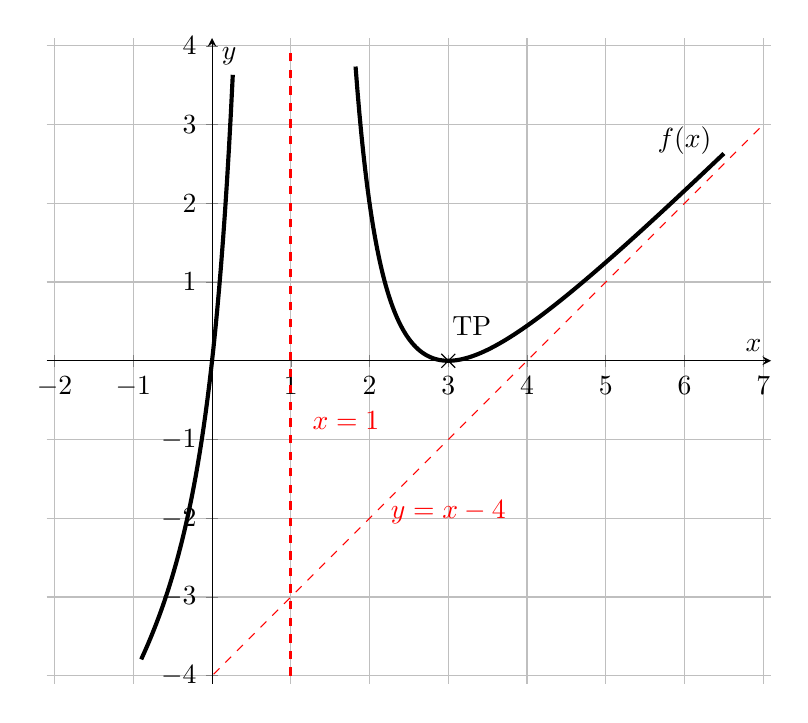
\begin{tikzpicture}
    \begin{axis}
[restrict y to domain=-4:4, axis x line=center, axis y line=center,%
 x=1cm,y=1cm,
    xmin= -2.1, xmax = 7.1,
    ymin= -4.1, ymax=4.1,
        axis lines = middle, 
        ymajorgrids=true,
        xmajorgrids=true,
        xtick={-2,  ..., 7},
        ytick={-4, ..., 4},
        xlabel = $x$,
        ylabel=$y$]
        \addplot[color= black, samples = 300, domain= -0.9:6.5,line width=1.5pt]{((x^3-6*x^2+9*x) / (x^2 -2*x +1)};
        \addplot[color= red, dashed, samples = 300, domain= -0.1:7]{x - 4};
        \draw [ red,dashed,line width=1pt] (1,-4) -- (1,4);
        \draw (-3,-1.3)   node [above] {NS};
        \draw (3,0) -- ++(-2.5pt,-2.5pt) -- ++(5pt,5pt) ++(-5pt,0pt) -- ++(5pt,-5pt);
         \draw (3.3,0.2)   node [above] {TP};
        \draw (6,2.5)   node [above] {$f(x)$};
        \draw[red] (3,-2.2)   node [above] {$y = x-4$};
        \draw[red] (1.7,-1)   node [above] {$x=1$};
        
    \end{axis}
\end{tikzpicture}
\end{center}
 \end{enumerate}
 \end{bsp}
 \begin{b8d}{Definitionslücken}{}
Während der Kurvendiskussion müssen die Definitionslücken immer beachtet werden. Das bedeutet, dass sowohl bei der Monotonietabelle als auch bei der Krümmungstabelle die Definitionslücke berücksichtigt werden müssen. An der Definitionslücke kann sich sowohl die Monotonie als auch die Krümmung ändern.
 \end{b8d}
 Die Grenzwertbetrachtungen können nach der Fallunterscheidung \ref{Fallgebrochenrational} bestimmt werden.
  \subsection{Wurzelfunktionen}
  \subsubsection{Die Umkehrfunktion}
  Einfache Wurzelfunktionen können als Umkehrfunktion der quadratischen Funktion betrachtet werden. Hierbei ist es notwendig, dass die Umkehrfunktion und die notwendigen Bedingungen der Umkehrbarkeit definiert werden. \index{Funktionen!Wurzelfunktion!Umkehrfunktion}
  \begin{defi}{Umkehrbarkeit eine Funktion}{}
Eine Funktion $f$ heißt umkehrbar, wenn verschiedene x-Werte des Definitionsbereichs $\mathds{D}_f$ stets verschiedene Funktionswerte $f(x)$ der Wertemenge $ \mathds{W}_f$ haben. Hierbei wird diese eindeutig umgekehrte Zuordnung Umkehrfunktion $f^{-1}$ genannt.
  \end{defi}
\begin{merke}{Kriterium für die Umkehrbarkeit}{}
Eine Funktion $f$ ist in einem Intervall $I\in \mathds{D}_f$ umkehrbar, genau dann wenn die Funktion im Intervall $I$ streng monoton ist. 
\end{merke}
\begin{b8d}{Eigenschaften von Umkehrfunktionen}{}
Bildet man die Umkehrfunktion einer umkehrbaren Funktion $f$ vertauschen sich der Definitionsbereich und der Wertebereich. Es gilt damit der folgende Zusammenhang: $$\mathds{D}_f = \mathds{W}_{f^{-1}}$$ und $$\mathds{W}_{f} = \mathds{D}_{f^{-1}}$$
Die Umkehrfunktion $f^{-1}$ kann durch eine Spiegelung des Graphen $G_f$ der Funktion $f$ an der Winkelhalbierenden $y= x$ gebildet werden.
\end{b8d}
\begin{b8d}{Bestimmung der Umkehrfunktion}{}
Die Bestimmung der Umkehrfunktion erfolgt in zwei Schritten. Als erstes muss man ein Intervall finden in der die gegebene Funktion umkehrbar ist und dann vertauscht man die x- und y- Koordinate und stellt nach y - Koordinate um. Als Beispiel wird die Umkehrfunktion $f^{-1}$ der Funktion $f(x) = x^2+4x+6$ gebildet.
\begin{enumerate}
    \item Finden eines Intervalls, in dem die Funktion umkehrbar ist. Damit die Funktion umkehrbar ist muss ein Intervall $I \ in \mathds{D}_f$ gefunden werden, indem die Funktion streng monoton ist.
    \begin{equation*}
        \begin{split}
            f(x)&= x^2+4x+6 \\
            f'(x)&= 2x+4\\
            0&= 2x+4 \hspace{0.5cm} | -4\\
            2x&= -4 \hspace{0.5cm} | :2\\
            x&= -2
        \end{split}
    \end{equation*}
    Für das Intervall $I$ folgt damit $I_1=]-\infty; -2[ $ bzw. $I_2 = ]-2;\infty[$. Damit ist $f$ im Intervall $I_1$ bzw. $I_2$ umkehrbar.
    \item Für die Umkehrfunktion $f^{-1}$ wird das Intervall $I_1 = ]-\infty; -2[$ gewählt. Das bedeutet, dass die Funktion $f(x) = x^2+4x+6$ mit $\mathds{D}_f = ]-\infty; -2[$ und $\mathds{W}_f = [2, \infty[$ betrachtet wird.
    \begin{equation*}
        \begin{split}
            y &= x^2+4x+6\\
            y &= (x+2)^2 +2 \hspace{0.5cm}| \hspace{0.25cm} \text{Vertauschung von x und y} \\
            x &= (y+2)^2+2 \hspace{0.5cm}| -2 \\
            x-2 &= (y+2)^2 \hspace{0.5cm}| \hspace{0.15cm}\sqrt{\hspace{0.15cm}} \hspace{0.15cm}\text{(Vorzeichen der Wurzel ist negativ aufgrund des Intervalls}\hspace{0.15cm} I_1)\\
            -\sqrt{x-2} &=y+2 \hspace{0.5cm}| -2\\
            y=f^{-1}(x) &= -2-\sqrt{x-2}
        \end{split}
    \end{equation*}
    Damit ergibt sich für die Umkehrfunktion $f^{-1}(x) = -2-\sqrt{x-2}$ und $\mathds{D}_{f^{-1}} =  \mathds{W}_f = [2, \infty[$ und $\mathds{W}_{f^{-1}}=\mathds{D}_f = ]-\infty; -2[ $
\end{enumerate}
\begin{center}
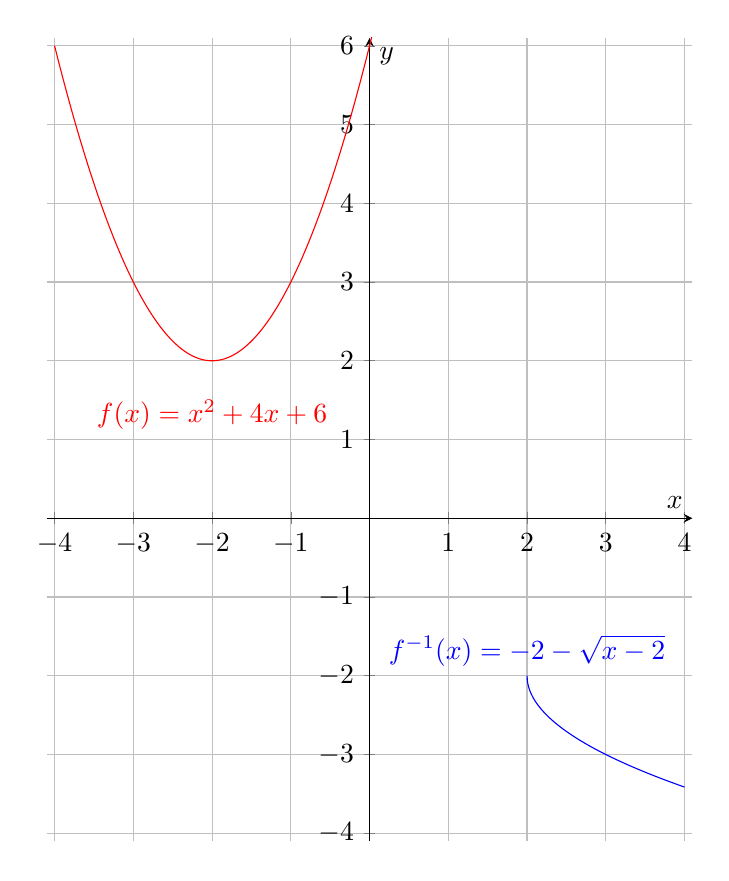
\begin{tikzpicture}
    \begin{axis}[xmin= -4.1, xmax = 4.1, ymin= -4.1, ymax=6.1,
    x=1cm,y=1cm,
        axis lines = middle, 
        ymajorgrids=true,
        xmajorgrids=true,
        xtick={-4, -3, -2,  ..., 4},
        ytick={ -4, ..., 6},
        xlabel = $x$,
        ylabel=$y$]
        \addplot[color= red, samples = 500, domain= -4:4]{x^2 +4*x+6};
        \draw[red] (-2,1)   node [above] {$f(x) = x^2+4x+6$};
       \addplot[color= blue, samples = 500, domain= 2:4]{-2-(x-2)^(0.5)};
      
        \draw[blue] (2,-2)   node [above] {$f^{-1}(x)= -2-\sqrt{x-2}$};

    \end{axis}
\end{tikzpicture}
\end{center}
\end{b8d}
 \subsubsection{Die allgemeine Wurzelfunktion}\index{Funktionen!Wurzelfunktion!allgemeine Wurzelfunktion}
 Der Graph der einfachen Wurzelfunktion $f(x) = \sqrt{x}$ geht durch die Spiegelung der Normalparabel an der Winkelhalbierenden $y=x$ hervor. Die allgemein Wurzelfunktion $f(x) = a\cdot \sqrt{x-b} +c$ ergibt sich dann durch lineare Transformationen der einfachen Wurzelfunktion.
 \begin{satz}{Die allgemeine Wurzelfunktion}{}
Der Graph der Funktion $f(x) = a\cdot \sqrt{x-b}+c$ und $x\geq b$ ist eine Halbparabel und ergibt sich durch folgende lineare Transformationen aus der allgemeinen Wurzelfunktion $g(x)= \sqrt{x}$ wie folgt:
\begin{itemize}
    \item Verschiebung um b in x-Richtung
    \item Strecken bzw. Stauchen mit dem Faktor a in y-Richtung
    \item Verschiebung um c in y-Richtung
\end{itemize}
 \end{satz}
 \begin{center}
\begin{tikzpicture}
    \begin{axis}[xmin= -1.1, xmax = 6.1, ymin= -1.1, ymax=4.1,
    x=1cm,y=1cm,
        axis lines = middle, 
        ymajorgrids=true,
        xmajorgrids=true,
        xtick={-1,  ..., 6},
        ytick={ -1, ..., 4},
        xlabel = $x$,
        ylabel=$y$]      

        \addplot[red, samples = 500, domain= 2:6]{2 + 0.5*(x-2)^(0.5)};
        \draw[red] (3,3)   node [above] {$f(x)=\dfrac{1}{2} \cdot \sqrt{x-2} + 2$};
        \addplot[ samples = 500, domain= 0:6]{(x)^(0.5)};
         \draw (2,0.5)   node [above] {$f(x)= \sqrt{x}$};
    \end{axis}
\end{tikzpicture}
\end{center}
 Eine besondere Art von Wurzelfunktionen bilden die Halbkreise als Graphen von Wurzelfunktionen.
 \begin{merke}{Halbkreise als Graphen der Wurzelfunktion}{}
Alle Punkte $P(x|y)$ die auf einem Kreis mit Radius $r$ um den Ursprung des Koordinatensystems liegen, erfüllen die Gleichung $$x^2+y^2 = r^2.$$ Bei der Bildung der Umkehrfunktion $f^{-1}$ folgt für die den Graphen der Umkehrfunktion $G_{f^{-1}}$ der Term $f^{-1}(x) = \sqrt{r^2-x^2}$. Für die Werte $-r\leq x\leq r$ ergibt sich als Graph ein Halbkreis mit Radius $r$ um den Ursprung.
 \begin{center}
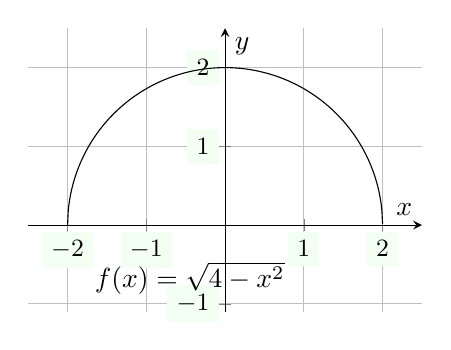
\begin{tikzpicture}
    \begin{axis}[xmin= -2.5, xmax = 2.5, ymin= -1.1, ymax=2.5,
    x=1cm,y=1cm,
        axis lines = middle, 
        ymajorgrids=true,
        xmajorgrids=true,
        xtick={-2,  ..., 2},
        ytick={ -1, ..., 2},
        xlabel = $x$,
        ylabel=$y$,
        ticklabel style={font=\small,fill=green!5},]      
        \addplot[samples = 500, domain= -2:2]{(4-x^2)^(0.5)};
        \draw (-0.45,-1)   node [above] {$f(x)= \sqrt{4-x^2}$};
      
    \end{axis}
\end{tikzpicture}
\end{center}
 \end{merke}
 \begin{merke}{Halbkreise mit beliebigen Mittelpunkt}{}
   Halbkreise um beliebige Mittelpunkte $M(a|b)$ lassen sich durch den Funktionsterm $$f(x)= \sqrt{r^2-(x-a)^2} + b $$ beschreiben. \\
   Das Beispiel beschreibt einen Halbkreis mit Radius $r=9$ um den Mittelpunkt $M(1,5|1)$.
   \begin{center}

   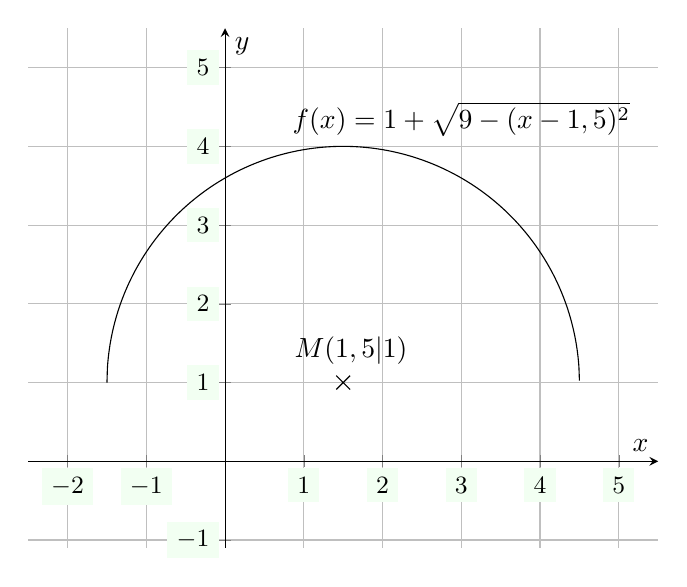
\begin{tikzpicture}
    \begin{axis}[xmin= -2.5, xmax = 5.5, ymin= -1.1, ymax=5.5,
    x=1cm,y=1cm,
        axis lines = middle, 
        ymajorgrids=true,
        xmajorgrids=true,
        xtick={-2,  ..., 5},
        ytick={ -1, ..., 5},
        xlabel = $x$,
        ylabel=$y$,
        ticklabel style={font=\small,fill=green!5}]      
         \addplot[smooth,samples= 1000,domain=-1.4999999695999992:4.4999999531379]{(3^2-(x-1.5)^2)^(0.5) +1};
        \draw (3,4)   node [above] {$f(x)= 1+\sqrt{9-(x-1,5)^2}$};
        \draw (1.5,1) -- ++(-2.5pt,-2.5pt) -- ++(5pt,5pt) ++(-5pt,0pt) -- ++(5pt,-5pt);
        \draw (1.6,1.1)   node [above] {$M(1,5|1)$};
    \end{axis}
\end{tikzpicture}
\end{center}
 \end{merke}
 \begin{bem}{Ableitung der Wurzel}{}
Die Ableitung einer Wurzelfunktion (Ableitungen der Wurzelfunktion findet man in \ref{Ableitungen}.) kann auf zwei unterschiedliche Arten erfolgen. Man verwendet entweder die Kettenregel mit der Wurzel als äußerer Funktion und dem Radikanden als innere Funktion oder wandelt die Wurzel in einen rationalen Exponenten um und wendet dann die Kettenregel an.
\begin{enumerate}
    \item Ableitung als Wurzel
    \begin{equation*}
        \begin{split}
            f(x) &= \dfrac{2}{3} \cdot \sqrt[3]{x^4-2x^3 +7x+2}\\
            f'(x) &= \dfrac{2}{3} \cdot \dfrac{1}{3} \dfrac{4x^3-6x^2+7}{\sqrt[3]{(x^4-2x^3 +7x+2)^2}} 
        \end{split}
    \end{equation*}
    \item Ableitung als rationale Funktion
    \begin{equation*}
        \begin{split}
            f(x) &= \dfrac{2}{3} \cdot \sqrt[3]{x^4-2x^3 +7x+2}\\
            &= \dfrac{2}{3} \cdot (x^4-2x^3+7x+2)^{\frac{1}{3}}\\
            f'(x) &= \dfrac{2}{3} \cdot \dfrac{1}{3} \cdot (x^4-2x^3+7x+2)^{-\frac{2}{3}} \cdot (4x^3-6x^2+7)
        \end{split}
    \end{equation*}
\end{enumerate}
 \end{bem}
 \subsection{Trigonometrische Funktionen}
Allgemeine Betrachtungen zum Sinus und Kosinus findet man im Anhang \ref{SinCos}. 
 \begin{defi}{Ableitungen von Sinus und Kosinus}{}\index{Funktionen!Trigonometrische!Ableitung}
Die Ableitungen der trigonometrischen Funktionen Sinus und Kosinus lauten wie folgt:
\begin{multicols}{2}
\noindent
\begin{equation*}
    \begin{split}
        f(x)&=\sin{(x)} \hspace{0.25cm}\text{mit} \hspace{0.25cm} \mathds{D}_f =  \mathds{R}\\
        f'(x)&= \cos{(x)} 
    \end{split}
    \end{equation*}
    \begin{equation*}
        \begin{split}
        g(x)&=\cos{(x)} \hspace{0.25cm}\text{mit} \hspace{0.25cm} \mathds{D}_g =  \mathds{R}\\
        g'(x)&= -\sin{(x)} 
    \end{split}
\end{equation*}
\end{multicols}
 \end{defi}
\begin{center}
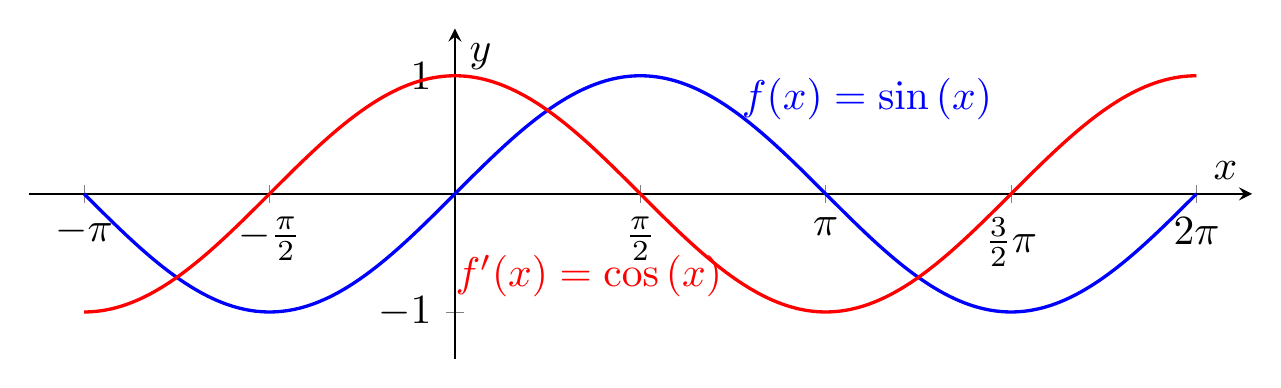
\begin{tikzpicture}[scale=1.5]
  \begin{axis}[
      axis lines = middle, 
      xlabel=$x$, 
      ylabel=$y$, 
      xmin=-180,xmax=360,ymin=-1,ymax=1,
      xtick = {-180,-90,...,360},     
      xticklabels = {$-\pi$,$-\frac{\pi}{2}$,0,$\frac{\pi}{2}$,$\pi$,$\frac{3}{2}\pi$,$2\pi$},
      ytick ={-1,0,1},
      yticklabels ={$-1$,$0$,$1$},
      enlarge x limits=.05,
      enlarge y limits=.2,
      y=1cm,% <- ergänzt
      x=0.017444cm,% <- ergänzt
      ]
\addplot[blue,thick,samples=300,domain=-180:360]{sin(x)};
\addplot[red,thick,samples=300,domain=-180:360]{cos(x)};

\draw[blue] (200,0.5)   node [above] {$f(x)= \sin{(x)}$};
\draw[red] (65,-1)   node [above] {$f'(x)= \cos{(x)}$};
\end{axis}
\end{tikzpicture} 
\end{center}
\begin{center}
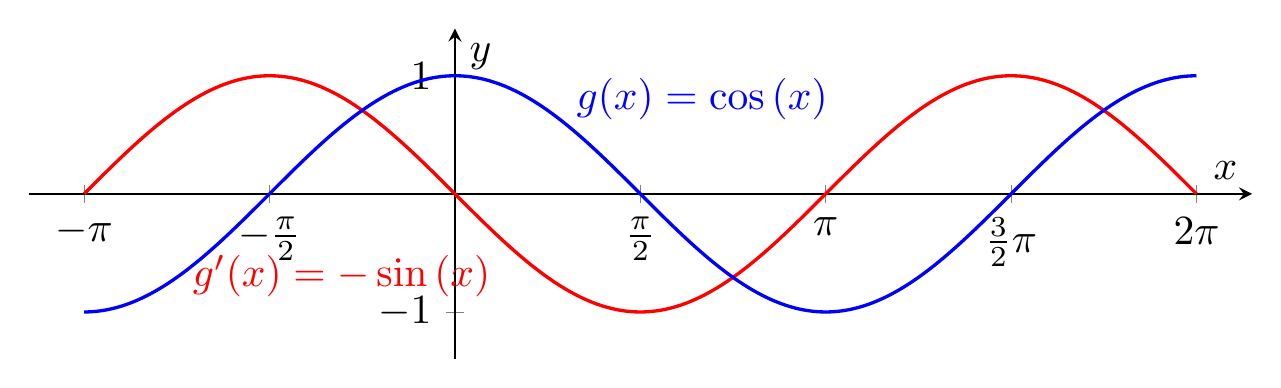
\begin{tikzpicture}[scale=1.5]
  \begin{axis}[
      axis lines = middle, 
      xlabel=$x$, 
      ylabel=$y$, 
      xmin=-180,xmax=360,ymin=-1,ymax=1,
      xtick = {-180,-90,...,360},     
      xticklabels = {$-\pi$,$-\frac{\pi}{2}$,0,$\frac{\pi}{2}$,$\pi$,$\frac{3}{2}\pi$,$2\pi$},
      ytick ={-1,0,1},
      yticklabels ={$-1$,$0$,$1$},
      enlarge x limits=.05,
      enlarge y limits=.2,
      y=1cm,% <- ergänzt
      x=0.017444cm,% <- ergänzt
      ]
\addplot[red,thick,samples=300,domain=-180:360]{-sin(x)};
\addplot[blue,thick,samples=300,domain=-180:360]{cos(x)};
\draw[blue] (120,0.5)   node [above] {$g(x)= \cos{(x)}$};
\draw[red] (-55,-1)   node [above] {$g'(x)= - \sin{(x)}$};
\end{axis}
\end{tikzpicture} 
\end{center}
Wie in \ref{SinCos} dargestellt wurde ergibt sich der Tangens als Quotient von $\sin$ und $\cos$ und damit lautet die Ableitung des Tangens wie folgt.
\begin{satz}{Ableitung des Tangens}{} \index{Ableitungsregeln!Tangensfunktion}\index{Funktionen!Tangens!Ableitung}
Die Funktion $f$ mit $ f(x)= \tan{(x)} = \dfrac{\sin{(x)}}{\cos{(x)} }$ mit $\mathds{D}_f = \mathds{R}\setminus\{\dfrac{\pi}{2} + k\cdot \pi\}$ und $ k \in \mathds{N} $ wird mit Hilfe der Quotientenregel abgeleitet. Es ergibt sich damit folgende Ableitungsfunktion: 
\begin{equation*}
    \begin{split}
    f'(x) &= \dfrac{\cos{(x)} \cdot \cos{(x)} - \sin{(x)} \cdot (-\sin{(x)})}{(\cos{(x)})^2}\\
    &= \dfrac{(\cos{(x)})^2+ (\sin{(x)})^2 }{(\cos{(x)})^2} \hspace{0.5cm}| \hspace{0.15cm}\text{Trigonometrischen Pythagoras}\\
    &= \dfrac{\cos^2{(x)} + \sin^2{(x)}}{\cos^2{(x)}}\\
    &= \dfrac{1}{\cos^2{(x)}}
    \end{split}
\end{equation*}
\begin{center}
    
\begin{tikzpicture}
  \begin{axis}[
      axis lines = middle, 
      xlabel=$x$, 
      ylabel=$y$, 
      xmin=-180,xmax=360,ymin=-4.1,ymax=4.1,
      xtick = {-180,-90,...,360},     
      xticklabels = {$-\pi$,$-\frac{\pi}{2}$,0,$\frac{\pi}{2}$,$\pi$,$\frac{3}{2}\pi$,$2\pi$},
      ytick ={-4,-3,-2,-1,0,1,2,3,4},
      yticklabels ={$-4$,$-3$,$-2$,$-1$,$0$,$1$,$2$,$3$,$4$},
      %enlarge x limits=.05,
      %enlarge y limits=.2,
      y=1cm,% <- ergänzt
      x=0.017444cm,% <- ergänzt
      ticklabel style={font=\small,fill=green!5}]
      \addplot[red,thick,samples=300,domain=-180 : -91]{tan(x)};
\addplot[red,thick,samples=300,domain=-90 : 89]{tan(x)};
\addplot[red,thick,samples=300,domain=91 : 269]{tan(x)};
\addplot[red,thick,samples=300,domain=271 : 360]{tan(x)};
\addplot[blue,thick,samples=300,domain=-70 : 70]{1/((cos(x))^2)};
\addplot[blue,thick,samples=300,domain=110 : 250]{1/((cos(x))^2)};
\addplot[blue,thick,samples=300,domain=290 : 350]{1/((cos(x))^2)};
\addplot[blue,thick,samples=300,domain=-179 : -100]{1/((cos(x))^2)};
\draw [red,dashed,line width=0.5pt] (-90,-4) -- (-90,4);
\draw[blue] (120,0.15)   node [above] {$f'(x)= \dfrac{1}{\cos^2{(x)}}$};
\draw[red] (65,-1)   node [above] {$f(x)= - \tan{(x)}$};

\end{axis}
\end{tikzpicture} 
\end{center}
\end{satz}
\begin{b8d}{Eigenschaften der Sinus- und Kosinuskurve}{}
Für die Kurvendiskussion trigonometrischer Funktionen und der darin vorkommenden Lösung von trigonometrischer Gleichungen ist es wichtig, dass die allgemeinen Eigenschaften der Sinus- und Kosinuskurve bekannt sind. Insbesondere ist der Merksatz \ref{SinCosEigenschaften} zu beachten.
\end{b8d}
\begin{bsp}{Kurvendiskussion einer trigonometrischen Funktion}{}\index{Funktionen!Trigonometrische!Kurvendiskussion}
Es soll am Beispiel der Funktion $f$ mit $f(x) = -2\sin{(2(x-\frac{\pi}{3}))} +2$  mit $\mathds{D}_f = \mathds{R}$ eine Kurvendiskussion durchgeführt werden.
\begin{enumerate}
\item Eigenschaften des Graphen anhand des Funktionsterms:
\begin{itemize}
    \item $b=\dfrac{\pi}{3} \longrightarrow$ Verschiebung um $\dfrac{\pi}{3}$  entlang der x-Achse
    \item $b=2 \longrightarrow$ Änderung der Periode zu $p= \dfrac{2\pi}{2} = \pi$ (Stauchung)
    \item $a = 2 \longrightarrow$ Streckung entlang der y-Achse mit Faktor 2 (Änderung der Amplitude)
    \item Vorfaktor $-1 \longrightarrow$ Spiegelung an der x-Achse
    \item $d= 2 \longrightarrow $ Verschiebung um 2 entlang der y-Achse
\end{itemize}
    \item Symmetrie der Funktion:
    \begin{equation*}
        \begin{split}
            f(-x) &=  -2\sin{(2((-x)-\frac{\pi}{3}))} +2\\
            &=  -2\sin{(-2x-2\cdot \frac{\pi}{3})} +2\\
            &\neq f(x)\\
            &\neq -f(x)
        \end{split}
    \end{equation*}
    Damit ist die Funktion $f(x)$ weder achsensymmetrisch zu y-Achse noch punktsymmetrisch zum Ursprung.
    \item Nullstellen:\begin{itemize}
        \item Schnittpunkte mit der x-Achse
    \begin{equation*}
        \begin{split}
            f(x) &= 0\\
            0 &=  -2\sin{(2(x-\frac{\pi}{3}))} +2 \hspace{0.5cm} | -2\\
            -2 &=  -2\sin{(2(x-\frac{\pi}{3}))}\hspace{0.5cm} | :(-2)\\
            1 &= \sin{(2(x-\frac{\pi}{3}))} \hspace{0.5cm} | \arcsin{ ()} \hspace{0.2cm} \text{siehe hierfür Merksatz \ref{SinCosEigenschaften}} \\ 
            \dfrac{1}{2}\pi +2\cdot k \pi &= 2(x-\frac{\pi}{3}) \hspace{0.5cm} | : 2\\
            \dfrac{1}{4}\pi +k\pi &= x-\frac{\pi}{3}\hspace{0.5cm}| + \frac{\pi}{3}\\
            \dfrac{7}{12} \pi +k\pi &= x \hspace{0.5cm}|\text{ mit } k\in \mathds{Z}
            \end{split}
            \end{equation*}
            Es folgt damit für die Nullstellen, dass alle $x_k=\dfrac{7}{12} \pi +k\pi$ mit $k\in \mathds{Z}$ die Nullstellengleichung erfüllen.
            \item Schnittpunkt mit der y-Achse
            \begin{equation*}
                \begin{split}
                    f(0) &= -2\sin{(2(0-\frac{\pi}{3}))} +2\\
                    &= -2\sin{(-2\frac{\pi}{3})} +2\\
                    &= -2\cdot( -\dfrac{\sqrt{3}}{2} )+2\\
                    &= \sqrt{3} +2 \approx 3,73
                \end{split}
            \end{equation*}
            \end{itemize}
            \item Ableitungen: \begin{equation*}
                \begin{split}
                    f(x) &= -2\sin{(2(x-\frac{\pi}{3}))} +2\\
                    f'(x) &= -2\cos{(2(x-\frac{\pi}{3}))} \cdot 2\\
                    &= -4\cos{(2(x-\frac{\pi}{3}))}\\
                    f''(x) &= 4\sin{(2(x-\frac{\pi}{3}))}\cdot 2\\
                    &= 8\sin{(2(x-\frac{\pi}{3}))} 
                \end{split}
            \end{equation*}
            \item Berechnung der Extrema:
            \begin{equation*}
                \begin{split}
                    0&= -4\cos{(2(x-\frac{\pi}{3}))} \hspace{0.5cm} | :(-4)\\
                    0&= \cos{(2(x-\frac{\pi}{3}))}\hspace{0.5cm} | \arccos{()}\\
                    \dfrac{\pi}{2} + k\pi &= 2(x-\frac{\pi}{3}) \hspace{0.5cm} |:2\\
                    \dfrac{\pi}{4} +\dfrac{k\pi}{2} &=x-\frac{\pi}{3} \hspace{0.5cm}| +\frac{\pi}{3}\\
                    \dfrac{7}{12}\pi + \dfrac{k\pi}{2} &= x
                \end{split}
            \end{equation*}
             Es folgt damit für die Nullstellen von $f'(x)$, dass alle $x_k=\dfrac{7}{12} \pi +\dfrac{k\pi}{2}$ mit $k\in \mathds{Z}$ die Nullstellengleichung erfüllen.
Die Art der Extremstellen muss dann für spezielle Werte von $k$ geprüft werden.
\item Nullstellen der zweiten Ableitung:
\begin{equation*}
    \begin{split}
        0&= 8\sin{(2(x-\frac{\pi}{3}))}\hspace{0.5cm} | :8\\
        0&= \sin{(2(x-\frac{\pi}{3}))}\hspace{0.5cm} | \arcsin{()}\\
        k\pi&= 2(x-\frac{\pi}{3}) \hspace{0.5cm} | :2\\
        \dfrac{k\pi}{2} &= x-\frac{\pi}{3} \hspace{0.5cm} |+\frac{\pi}{3}\\
        \dfrac{k\pi}{2} +\frac{\pi}{3} &= x
    \end{split}
\end{equation*}
             Es folgt damit für die Nullstellen von $f''(x)= \dfrac{k\pi}{2} +\dfrac{\pi}{3}$, dass alle $x_k=$ mit $k\in \mathds{Z}$ die Nullstellengleichung erfüllen.
Das eigentliche Krümmungsverhalten muss dann für spezielle Werte von $k$ ermittelt werden.

\item Graph der Funktion $f(x) = -2\cdot \sin{(2\cdot (x-\frac{\pi}{3}))} +2$ im Intervall $I=[-\pi; \frac{3}{2}\pi]$:
\begin{center}
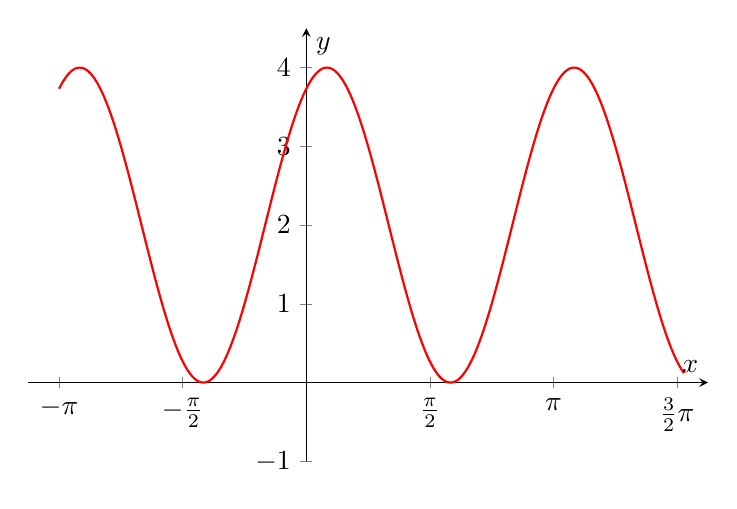
\begin{tikzpicture}
  \begin{axis}[
      axis lines = middle, 
      xlabel=$x$, 
      ylabel=$y$, 
      xmin=-180,xmax=270,ymin=-1,ymax=4.5,
      xtick = {-180,-90,...,270},     
      xticklabels = {$-\pi$,$-\frac{\pi}{2}$,0,$\frac{\pi}{2}$,$\pi$,$\frac{3}{2}\pi$},
      ytick ={-1,0,1,2,3,4},
      yticklabels ={$-1$,$0$,$1$,$2$, $3$, $4$},
      enlarge x limits=.05,
      %enlarge y limits=.2,
      y=1cm,% <- ergänzt
      x=0.017444cm,% <- ergänzt
      ]
\addplot[red,thick,smooth,samples = 500,domain=-180:275]{-2*sin(2*(x-60))+2};
\end{axis}
\end{tikzpicture} 
\end{center}
\end{enumerate}
    \end{bsp}
 \subsection{Exponentialfunktionen}\index{Funktionen!e-Funktion}
 In der Mathematik wird unter dem Begriff der natürlichen Exponentialfunktion bzw. der $e$-Funktion folgende Funktion verstanden $$f(x) = e^x$$ mit $\mathds{D}_f = \mathds{R}$ und $\mathds{W}_f =\mathds{R}^{+}$.
\begin{center}
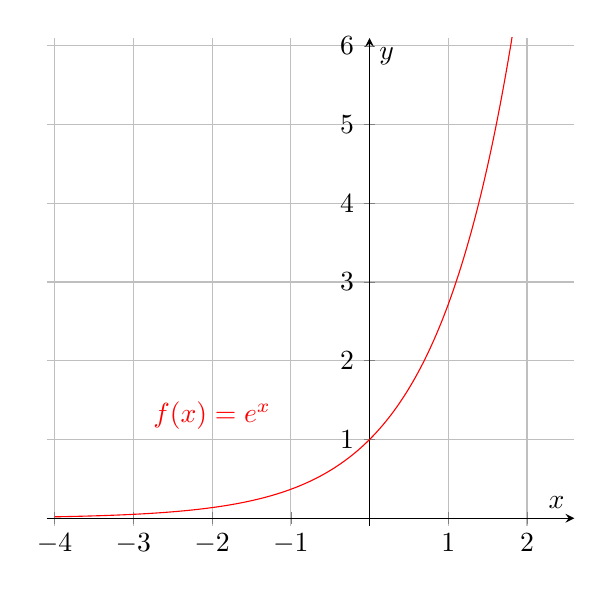
\begin{tikzpicture}
    \begin{axis}[xmin= -4.1, xmax = 2.6, ymin= -0.1, ymax=6.1,
    x=1cm,y=1cm,
        axis lines = middle, 
        ymajorgrids=true,
        xmajorgrids=true,
        xtick={-4, -3, -2,  ..., 2},
        ytick={ 0, ..., 6},
        xlabel = $x$,
        ylabel=$y$]
        \addplot[color= red, samples = 500, domain= -4:4]{e^x};
    \draw[red] (-2,1)   node [above] {$f(x) = e^x$};
    \end{axis}
\end{tikzpicture}
\end{center}
\subsubsection{Allgemeines zur $e$-Funktion}
\begin{satz}{Die Euler'sche Zahl e}{}
Die Zahl $e=2,71828...$ ist eine irrationale Zahl und ergibt sich durch folgenden Grenzwert: $$e= \lim_{n\longrightarrow \infty} \left(1+ \dfrac{1}{n}\right)^n.$$ Der Grenzwert konvergiert damit gegen den Wert von $e$.   
\end{satz}
Die $e$-Funktion ist eine Exponentialfunktion mit spezieller Basis und wird häufig verwendet, um natürliche Prozesse zu beschreiben. Die Umkehrfunktion der $e$-Funktion bildet die natürliche Logarithmusfunktion $g(x) = \ln{(x)}$. Siehe hierfür \ref{ln}
\begin{center}
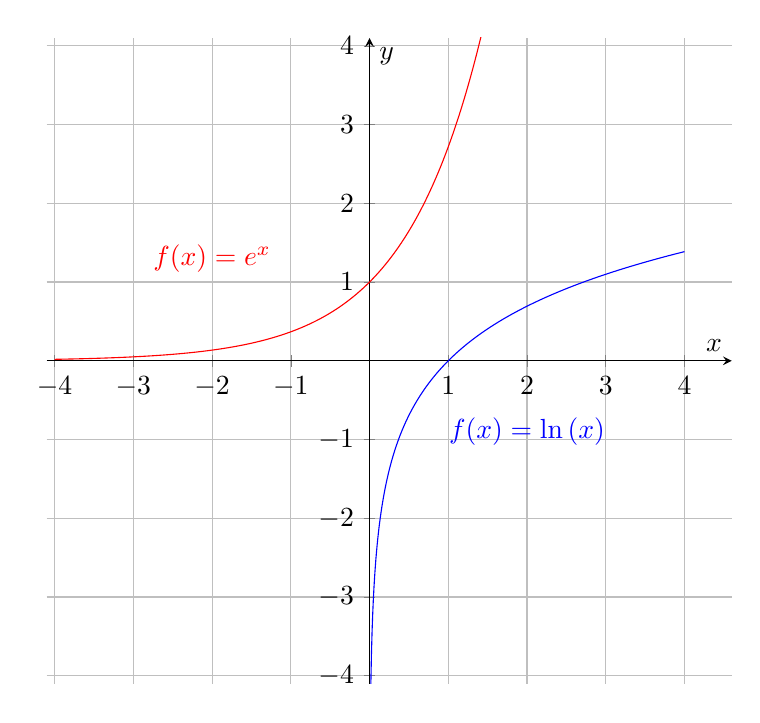
\begin{tikzpicture}
    \begin{axis}[xmin= -4.1, xmax = 4.6, ymin= -4.1, ymax=4.1,
    x=1cm,y=1cm,
        axis lines = middle, 
        ymajorgrids=true,
        xmajorgrids=true,
        xtick={-4, -3, -2,  ..., 4},
        ytick={ -4, ..., 4},
        xlabel = $x$,
        ylabel=$y$]
        \addplot[color= red, samples = 500, domain= -4:2]{e^x};
    \draw[red] (-2,1)   node [above] {$f(x) = e^x$};
    \addplot[color= blue, samples = 500, domain= 0:4]{ln(x)};
    \draw[blue] (2,-1.2)   node [above] {$f(x) = \ln{(x)}$};
    \end{axis}
\end{tikzpicture}
\end{center}
\begin{bem}{Grenzwerte der $e$-Funktion}{}\index{Funktionen!e-Funktion!Grenzwert}
Für die Funktion $f(x) = e^x$ mit $\mathds{D}_f = \mathds{R}$ gelten folgende Grenzwerte: $$\lim_{x\longrightarrow \infty} e^x = \infty$$ und $$\lim_{x\longrightarrow -\infty} e^x = 0$$ 
\end{bem}
\begin{satz}{Grenzwertverhalten der $e$-Funktion}{}
In Kombination mit Potenzfunktionen wächst die $e$-Funktion schneller als jede Potenzfunktion. Insbesondere gilt der Grenzwert $$\lim_{x\longrightarrow \infty} \dfrac{x^n}{e^x} = 0$$ für jedes $n\in \mathds{N}$.
\end{satz}
\begin{satz}{Ableitung der $e$-Funktion}{}\index{Funktionen!e-Funktion!Ableitung}
Die natürliche Exponentialfunktion besitzt die Eigenschaft, dass die Funktion mit ihrer Ableitung übereinstimmt. Es gilt also folgendes $$f(x) = e^x = f'(x).$$
\end{satz}
\begin{satz}{Ableitungen spezieller $e$-Funktion}{}
Die $e$-Funktion tritt häufig mit anderen Funktionen verknüpft auf. So ist $f(x) = e^{g(x)}$ eine der häufigsten auftretenden Funktionen. Hierbei ist zu beachten, dass die Kettenregel für die Ableitung angewendet werden muss. Damit ergibt sich für die Ableitung $$f'(x) = e^{g(x)} \cdot g'(x).$$  Bei der Klasse von Funktionen $f(x) = e^x \cdot g(x)$ muss die Produktregel verwendet werden. Es folgt damit, dass $$f'(x) = e^x \cdot g(x) + e^x \cdot g'(x) = e^x\cdot (g(x)+ g'(x))$$ ist. Siehe hierfür im Anhang \ref{AbleitungEFunktion}
\end{satz}
 \subsubsection{Kurvendiskussion einer e-Funktion}\index{Funktionen!e-Funktion!Kurvendiskussion}
 Die Kurvendiskussion einer verknüpften $e$-Funktion erfolgt nach dem selben Muster wie die restlichen Funktionsklassen. Als Beispiel soll hier die Funktion $f(x) = 4x^2\cdot e^x$ betrachtet werden.
 \begin{bsp}{Kurvendiskussion der $e$-Funktion}{}
Gegeben ist die Funktion $f(x) = 4x^2\cdot e^x$ mit $\mathds{D}_f = \mathds{D}_{max}$
\begin{enumerate}
    \item Definitionsmenge: $\mathds{D}_f = \mathds{R}$ die Funktion ist damit auf ganz $\mathds{R}$ definiert.
    \item Symmetrie:
    \begin{equation*}
        \begin{split}
            f(-x) &= (-x)^2 \cdot e^{-x}\\
            &= x^2\cdot e^{-x}\\
            &\neq f(x)\\
            &\neq -f(x)
        \end{split}
    \end{equation*}
    Damit ist der Graph der Funktion $f(x)$ weder achsensymmetrisch zur y-Achse noch punktsymmetrisch zum Ursprung.
    \item Schnittpunkte mit den Koordinatenachsen:
    \begin{itemize}
        \item Nullstellen:
        \begin{equation*}
            \begin{split}
                0 &=f(x)\\
               0 &= 4x^2\cdot e^x\hspace{0.5cm}|\hspace{0.1cm} e^x >0 \text{ für alle} x \in \mathds{R}\\
               0 &=4x^2\\
               x_{1/2} &= 0
            \end{split}
        \end{equation*}
        Damit befindet sich bei $x=0$ eine doppelte Nullstelle.
        \item Schnittpunkt mit der y-Achse
        \begin{equation*}
            \begin{split}
                f(0)&= 4\cdot (0)^2 \cdot e^{0}\\
                &= 4\cdot 0 \cdot 1\\
                &= 0
            \end{split}
        \end{equation*}
    \end{itemize}
    Daraus folgt, dass der Graph $G_f$ der Funktion $f$ durch den Ursprung verläuft.
    \item Grenzwertverhalten:
    \begin{equation*}
            \begin{split}
               \lim_{x\longrightarrow \infty} f(x) &= \lim_{x\longrightarrow \infty} 4x^2\cdot e^x\\
               &=  \infty\\
               \lim_{x\longrightarrow -\infty} f(x) &= \lim_{x\longrightarrow -\infty} 4x^2\cdot e^x\\
               &= 0          
            \end{split}
        \end{equation*}
    \item Ableitungen:
    \begin{equation*}
            \begin{split}
               f(x) &= 4x^2\cdot e^x\\
               f'(x) &= 8x\cdot e^x + 4x^2 \cdot e^x\\
                    &= e^x \cdot (4x^2+8x)\\
                f''(x) &= e^x \cdot (4x^2+8x) + e^x \cdot (8x+8)\\
                 &= e^x\cdot (4x^2 +16x+8)
            \end{split}
        \end{equation*}
        \item Monotonie:
            \begin{equation*}
            \begin{split}
                f'(x)&=0\\
                0&= e^x \cdot (4x^2+8x) \hspace{0.5cm} | e^x \neq 0\\
                0&= 4x^2+8x\\
                &= x(4x+8)\\
                x_1 &= 0\\
                0&= 4x+8\hspace{0.5cm} | -8\\ 
                -8&= 4x \hspace{0.5cm} | :4\\
                x_2 &= -2
            \end{split}
        \end{equation*}
        \begin{center}\begin{tabular}{||c|c|c|c|c|c||}
    \hline
    $x$& $ -\infty <x<-2 $ & $ x =-2$ &$ -2<x<0 $ & $x=0 $& $ 0<x<\infty $\\
    \hline \hline
    $e^x$ & + & + & + & 1 & +  \\
    \hline
    $4x$ & - & - & - & 0 & + \\
     \hline
    $(x+2)$ & - & 0 & + & + & + \\
    \hline
    $f'(x)$ & + & 0 & - & 0 & +\\ 
    \hline
    \hline
    $G_f$ & smw & $HoP(-2|16\cdot e^{-2})$ & smf  & $TP(0|0)$& smw\\
    \hline
\end{tabular}
\end{center}
Berechnung der Koordinaten der Extrempunkte:
            \begin{equation*}
            \begin{split}
               f(0)&=0\\
               f(-2)&= 4(-2)^2 \cdot e^{-2}\\
               &=16\cdot e^{-2} \approx 2,17
            \end{split}
        \end{equation*}
        \item Krümmungsverhalten:
                \begin{equation*}
            \begin{split}
            f''(x)&= 0\\
               0 &=e^x\cdot (4x^2 +16x+8) \hspace{0.5cm} | e^x \neq 0\\
               0 &= 4\cdot (x^2 +4x+2)\\
               x_{1/2} &= \dfrac{-4\pm \sqrt{4^2 - 4\cdot 1\cdot 2}}{2\cdot 1}\\
               &= \dfrac{-4\pm \sqrt{16 - 8}}{2}\\
               &= \dfrac{-4\pm \sqrt{8}}{2}\\
               &= \dfrac{-4\pm 2\sqrt{2}}{2}\\
               &= -2\pm \sqrt{2}\\
               x_1&= -2+\sqrt{2} \approx -0,59\\
               x_2 &= -2-\sqrt{2} \approx -3,41           
            \end{split}
        \end{equation*}
                \begin{center}\begin{tabular}{||c|c|c|c|c|c||}
    \hline
    $x$& $ -\infty <x<x_2 $ & $ x =x_2$ &$ x_2<x<x_1 $ & $x=x_1 $& $ x_1<x<\infty $\\
    \hline \hline
    $4e^x$ & + & + & + & + & +  \\
    \hline
    $(x-x_2)$ & - & 0 & + & 0 & + \\
     \hline
    $(x-x_1)$ & - & - & - & + & + \\
    \hline
    $f''(x)$ & + & 0 & - & 0 & +\\ 
    \hline
    \hline
    $G_f$ & linksgekrümmt & $WP$ & rechtsgekrümmt  & $WP$& linksgekrümmt\\
    \hline
\end{tabular}
\end{center}
Berechnung der Koordinaten der Wendepunkte:
                \begin{equation*}
            \begin{split}
           f(-2-\sqrt{2})  &= (16\sqrt{2} +24) \cdot e^{-2-\sqrt{2}}\approx 1,53\\
           f(-2+\sqrt{2})  &= (-16\sqrt{2} +24) \cdot e^{-2+\sqrt{2}}\approx 0,76
            \end{split}
        \end{equation*}
        \item Graph:
        \begin{center}
    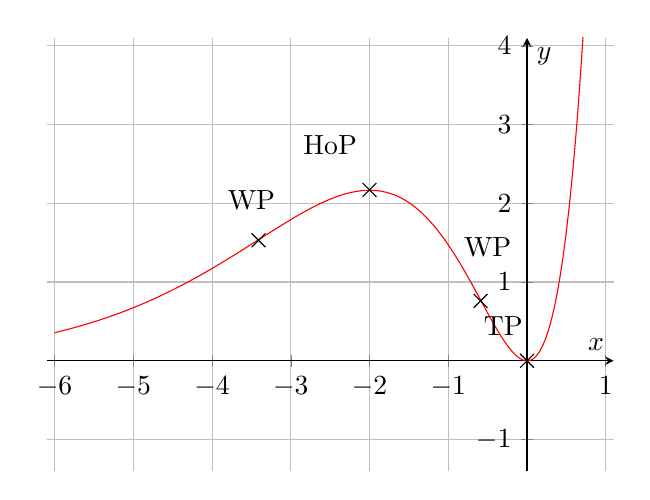
\begin{tikzpicture}
    \begin{axis}[xmin= -6.1, xmax = 1.1, ymin= -1.4, ymax=4.1,
    x=1cm,y=1cm,
        axis lines = middle, 
        ymajorgrids=true,
        xmajorgrids=true,
        xtick={-6, ..., 1},
        ytick={ -1, ..., 4},
        xlabel = $x$,
        ylabel=$y$]
        \addplot[color= red, samples = 500, domain= -6:1]{4*x^2*e^x};
        \draw (0,0) -- ++(-2.5pt,-2.5pt) -- ++(5pt,5pt) ++(-5pt,0pt) -- ++(5pt,-5pt);
         \draw (-0.3,0.2)   node [above] {TP};
         \draw (-2,2.17) -- ++(-2.5pt,-2.5pt) -- ++(5pt,5pt) ++(-5pt,0pt) -- ++(5pt,-5pt);
         \draw (-2.5,2.5)   node [above] {HoP};
         \draw (-3.41, 1.53) -- ++(-2.5pt,-2.5pt) -- ++(5pt,5pt) ++(-5pt,0pt) -- ++(5pt,-5pt);
         \draw (-3.5,1.8)   node [above] {WP};
        \draw (-0.59, 0.76) -- ++(-2.5pt,-2.5pt) -- ++(5pt,5pt) ++(-5pt,0pt) -- ++(5pt,-5pt);
         \draw (-0.5,1.2)   node [above] {WP};
    \end{axis}
\end{tikzpicture}
\end{center}
\end{enumerate}
 \end{bsp}
 \subsection{Logarithmusfunktionen}\index{Funktionen!Logarithmusfunktion}
 \subsubsection{Allgemeines zur $\ln{}$ Funktion}
 Die Logarithmusfunktion ist die Umkehrfunktion der $e$-Funktion. Damit ergibt sich für den Definitions- und Wertebereich folgende Zusmmenhänge.
 \begin{satz}{Die Logarithmusfunktion}{}
Die natürliche Logarithmusfunktion $f(x) = \ln{(x)}$ ordnet jeder positiven reellen Zahl den natürlichen Logarithmus zu. Für die Funktion gilt damit: $$\mathds{D}_f = \mathds{R}^+$$ und $$\mathds{W}_f = \mathds{R}.$$
 \end{satz}
 \begin{center}
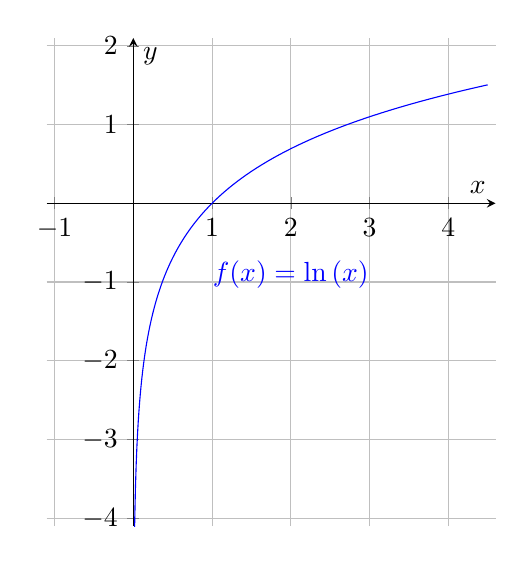
\begin{tikzpicture}
    \begin{axis}[xmin= -1.1, xmax = 4.6, ymin= -4.1, ymax=2.1,
    x=1cm,y=1cm,
        axis lines = middle, 
        ymajorgrids=true,
        xmajorgrids=true,
        xtick={-1,  ..., 4},
        ytick={ -4, ..., 2},
        xlabel = $x$,
        ylabel=$y$]       
    \addplot[color= blue, samples = 500, domain= 0:4.5]{ln(x)};
    \draw[blue] (2,-1.2)   node [above] {$f(x) = \ln{(x)}$};
    \end{axis}
\end{tikzpicture}
\end{center}
\begin{bem}{Grenzwerte der $\ln$-Funktion}{}\index{Funktionen!Logarithmusfunktion!Grenzwert}
Für die Funktion $f(x) = \ln{(x)}$ mit $\mathds{D}_f = \mathds{R}^+$ gelten folgende Grenzwerte:
$$\lim_{x \longrightarrow 0^+} f(x) = \lim_{x \longrightarrow 0^+} \ln{(x)} = -\infty$$ und $$\lim_{x \longrightarrow \infty} f(x) = \lim_{x \longrightarrow \infty} \ln{(x)} = \infty$$
\end{bem}
\begin{satz}{Grenzwertverhalten der $\ln{}$-Funktion}{}
In Kombination mit Potenzfunktionen wächst die $\ln{}$-Funktion langsamer als jede Potenzfunktion. Insbesondere gilt der Grenzwert $$\lim_{x\longrightarrow \infty} \dfrac{\ln{(x)}}{x^n} = 0$$ für jedes $n\in \mathds{N}$.
\end{satz}
\begin{satz}{Ableitung der $\ln$-Funktion}{} \index{Funktionen!Logarithmusfunktion!Ableitung}
Die natürliche Logarithmusfunktion $f(x) = \ln{(x)}$ besitzt folgende Ableitung: $$f'(x) = \dfrac{1}{x}$$ für alle $x\in \mathds{R}^+$
\end{satz}
\begin{satz}{Ableitungen spezieller $\ln$-Funktion}{}
Die $\ln$-Funktion tritt häufig mit anderen Funktionen verknüpft auf. So ist $f(x) = \ln{g(x)}$ eine der häufigsten auftretenden Funktionen. Hierbei ist zu beachten, dass die Kettenregel für die Ableitung angewendet werden muss. Damit ergibt sich für die Ableitung $$f'(x) = \dfrac{1}{ g(x)} \cdot g'(x) = \dfrac{g'(x)}{g(x)}.$$  
Bei der Klasse von Funktionen $f(x) = \ln{x} \cdot g(x)$ muss die Produktregel verwendet werden. Es folgt damit, dass
$$f'(x) = \dfrac{1}{x}\cdot g(x) +\ln{(x)} \cdot g'(x)$$ 
ist. Siehe hierfür im Anhang \ref{AbleitungEFunktion}
\end{satz}
 \subsubsection{Kurvendiskussion einer $\ln$-Funktion}
 Die Kurendiskussion einer $\ln$-Funktion unterscheidet wird anhand folgendes Beispiel kurz erläutert.
 \begin{bsp}{Kurvendiskussion einer $\ln$-Funktion}{ }
Gegeben ist die Funktion $f$ mit $f(x) = x^2\cdot \ln{(x)}$ und $\mathds{D}_f = \mathds{D}_{max}$.
\begin{enumerate}
    \item Definitionsbereich: Die Funktion $g(x) = \ln{(x)}$ ist nur für positive reelle zahlen definiert. Damit folgt für den Definitionsbereich der Funktion $f(x) = x^2\ln{(x)}$ folgendes: $\mathds{D}_f = \mathds{R}^+$.
    \item Symmetrie: Aufgrund des Definitionsbereichs ist es nicht nötig eine Untersuchung auf Symmetrie zum Ursprung bzw. zur y-Achse zu untersuchen.
    \item Nullstellen: 
        \begin{equation*}
            \begin{split}
                f(x) &=0\\
                0&= x^2\cdot \ln{(x)}\hspace{0.5cm} | \text{ Fallunterscheidung}\\
                0&= x^2\\
                x_{1/2} &= 0 \notin \mathds{D}_f\\
                0&= \ln{(x)}\\
                x_3&= 1
            \end{split}
        \end{equation*}
Schnittpunkte mit der y-Achse können aufgrund des Definitionsbereichs nicht existieren.
\item Ableitungen:
        \begin{equation*}
            \begin{split}
                f(x) &=x^2\cdot \ln{(x)}\\
                f'(x)&= 2x\cdot \ln{(x)} + x^2 \cdot \frac{1}{x}\\
                &=2x\cdot \ln{(x)} + x = x\cdot (2\cdot \ln{(x)} +1)\\
                f''(x) &= 2\cdot \ln{(x)} + 2x\cdot \frac{1}{x} +1\\
                &=2\cdot \ln{(x)} + 3
            \end{split}
        \end{equation*}

\item Monotonie:
        \begin{equation*}
            \begin{split}
                f'(x)&=0\\
               0&= x\cdot (2\cdot\ln{(x)} +1)\\
                x_1&= 0 \notin \mathds{D}_f\\
                0&= 2\cdot\ln{(x)} +1 \hspace{0.5cm} | -1\\
                 2\cdot\ln{(x)}&= -1 \hspace{0.5cm} | :2\\
                \ln{(x)}&= -\frac{1}{2} \hspace{0.5cm} |\hspace{0.2cm} e^{()} \text{ Anwendung der $e$-Funktion}\\
                x_2&= e^{-\frac{1}{2}}\approx 0,61
            \end{split}
        \end{equation*}
\begin{center}\begin{tabular}{||c|c|c|c|c|c||}
    \hline
    $x$& $ 0<x<e^{-\frac{1}{2}} $ & $ x =e^{-\frac{1}{2}}$ &$ e^{-\frac{1}{2}}<x<\infty $ \\
    \hline \hline
    $x$ & + & + & +   \\
    \hline
    $(\ln{(x)}+1)$ & - & 0 & +  \\
     \hline
    $f'(x)$ & - & 0 & + \\ 
    \hline
    \hline
    $G_f$ & smf & $TiP(e^{-\frac{1}{2}}|-\frac{1}{2} e^{-1})$ & smw  \\
    \hline
\end{tabular}
\end{center}
Berechnung der Lage des Extrempunktes:
        \begin{equation*}
            \begin{split}
               f(e^{-\frac{1}{2}}) &= (e^{-\frac{1}{2}})^2 \cdot \ln{(e^{-\frac{1}{2}})}\\
               &= \dfrac{1}{e} \cdot\left( -\dfrac{1}{2} \ln{(e)}\right)\\
                &= \dfrac{1}{e} \cdot \left(-\dfrac{1}{2}\right)
            \end{split}
        \end{equation*}
        \item Krümmungsverhalten:
        \begin{equation*}
            \begin{split}
                f''(x)&=0\\
               0&= 2\cdot \ln{(x)} + 3 \hspace{0.5cm} | - 3\\
               2\cdot \ln{(x)}&= -3 \hspace{0.5cm} | : 2\\
               \ln{(x)}&= -\dfrac{3}{2}  |\hspace{0.2cm} e^{()} \text{ Anwendung der $e$-Funktion}\\
               x&= e^{-\frac{3}{2} }\approx 0,22
            \end{split}
        \end{equation*}
        \begin{center}\begin{tabular}{||c|c|c|c|c|c||}
    \hline
    $x$& $ 0<x<e^{-\frac{3}{2}} $ & $ x =e^{-\frac{3}{2}}$ &$ e^{-\frac{3}{2}}<x<\infty $ \\
    \hline \hline
    $(2\ln{(x)}+3)$ & + & 0 & -  \\
     \hline
    $f''(x)$ & + & 0 & - \\ 
    \hline
    \hline
    $G_f$ & linksgekrümmt & $WP(e^{-\frac{3}{2}}|-\dfrac{3}{2} \cdot e^{-3})$ & rechtsgekrümmt \\
    \hline
\end{tabular}
\end{center}
Berechnung der Koordinaten des Wendepunktes:
\begin{equation*}
            \begin{split}
                f(e^{-\frac{3}{2}})&=\left(e^{-\frac{3}{2}}\right)^2 \cdot \ln{(e^{-\frac{3}{2}})}\\
            &= \dfrac{1}{e^3} \cdot \left(-\dfrac{3}{2} \ln{(e)}\right)\\
            &= \dfrac{1}{e^3} \cdot \left(-\dfrac{3}{2}\right)\\
               &= -\dfrac{3}{2} \cdot e^{-3}
            \end{split}
        \end{equation*}
\item Graph:
\begin{center}
 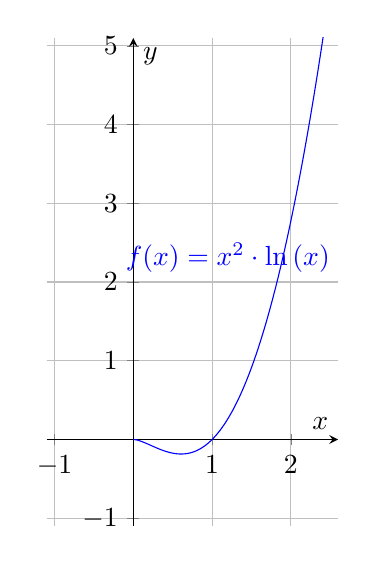
\begin{tikzpicture}
    \begin{axis}[xmin= -1.1, xmax = 2.6, ymin= -1.1, ymax=5.1,
    x=1cm,y=1cm,
        axis lines = middle, 
        ymajorgrids=true,
        xmajorgrids=true,
        xtick={-1,..., 2},
        ytick={ -1, ..., 5},
        xlabel = $x$,
        ylabel=$y$]       
    \addplot[color= blue, samples = 500, domain= 0.000000001:2.5]{x^2*ln(x)};
    \draw[blue] (1.2,2)   node [above] {$f(x) =x^2\cdot  \ln{(x)}$};
    \end{axis}
\end{tikzpicture}
\end{center}
\end{enumerate}
 \end{bsp}
 \section{Anwendungen der Differentialrechnung}
 \subsection{Modellierung von Funktionen}\index{Funktionen!Modellierung}
 Die Modellierung von Funktionen beschäftigt sich mit dem aufstellen von Funktionstermen. Hierbei werden Eigenschaften spezieller Funktionen vorgegeben und es sollen anhand dieser die Terme der entsprechenden Funktionen gefunden werden. Als Beispiel hierfür kann zum Beispiel das aufstellen einer quadratischen Funktion aufgrund des Scheitelpunktes und eines Punktes dienen.
 \begin{bsp}{}{}
Der Graph der quadratische Funktion soll folgende Eigenschaften haben:
\begin{itemize}
    \item Der Scheitelpunkt liegt bei $(-3|5)$
    \item Der Graph der Funktion geht durch den Punkt $P(1|2)$
\end{itemize}
Um den term zu finden wird als erstes die allgemeine Scheitelpunktform gewählt und die Koordinaten des Scheitelpunktes eingesetzt. So lautet die Scheitlepunktform $f(x) = a\cdot \left(x-x_S\right)^2 +y_S$. Nach dem einsetzen lautet der Term $f(x) = a\cdot \left(x-(-3)\right)^2 +5 = a\cdot \left(x+3\right)^2 +5 $. Um den Wert des Parameters a bestimmen zu können, muss der Punkt $P$ eingesetzt werden und dann wird nach $a$ aufgelöst.
\begin{equation*}
    \begin{split}
        2&= a\cdot (1+3)^2+5\\
        2&= a\cdot (4)^2 +5\\
        2&= a\cdot 16 +5 \hspace{0.5cm} | - 5\\
        -3&= a\cdot 16  \hspace{0.5cm} | : 16\\
        a&=-\dfrac{3}{16}
    \end{split}
\end{equation*}
Damit lautet der Term $f(x) = -\dfrac{3}{16} \cdot \left(x+3\right)^2 +5$.
 \end{bsp}
 Weitere häufig gebrauchte Beispiele sind das Aufstellen von Trigonometrischen  bzw. gebrochen-rationalen Funktionen. Bei diesen werden dann charakteristische Eigenschaften vorgegeben die dann verarbeitet werden müssen. 
 \subsection{Extremwertprobleme}\index{Extremwertprobleme}
 Bei Extremwertaufgaben werden Anwendungsaufgaben vorgegeben die durch eine Untersuchung der Monotonie gelöst werden sollen. Hierbei ist es möglich aus der Aufgabenstellungen mindestens zwei Gleichungen zu finden die in eine Funktion zusammengefasst werden muss.\\
 Diejenige Funktion die einen Extremwert annehmen soll wird hierbei als Zielfunktion bezeichnet. Die weiteren Funktionen werden als Nebenbedingungen bezeichnet.
 \begin{satz}{Extremwertaufgaben}{}
Hängt eine zu optimierende Größe von zwei oder mehreren variablen ab, müssen mithilfe von einer oder mehrere Nebenbedingungen eine oder mehrere Variablen aus dem zugehörigen Term eleminiert werden. Danach ist es möglich, das Extremum der Funktion mit einer Variablen zu bestimmen. Hierbei ist auf den Definitionsbereich zu achten.
 \end{satz}
 \begin{b8d}{Vorgehen beim lösen von Extremwertproblemen}{}
\begin{enumerate}
    \item Beschreiben der Größen, die extremal werden soll, durch einen Term, der mehrere Variablen enthalten kann.
    \item Formulierung von gegebenen Nebenbedingungen.
    \item Bestimmen der Zielfunktion, die nur noch von einer variablen abhängig ist.
    \item Untersuchung der Zielfunktion auf Extremwerte und Formulierung des Ergebnisses. Hierbei sind auch auf Randwerte zu achten.
\end{enumerate}
 \end{b8d}
 \begin{bsp}{Beispiel für Extremwertaufgaben}{}
Aus einem quadratischen Stück Pappe mit der festen Seitenlänge $a = 5\text{ cm}$ soll eine oben offene Schachtel hergestellt werden. Finde eine Funktionsgleichung für das Volumen der Schachtel in Abhängigkeit von der Länge $x$ (in cm) des Einschnitts und der allgemeinen Seitenlängen $a$. Für welchen Wert von $x$ wird das Volumen der Schachtel maximal. 
\begin{itemize}
    \item Zielfunktion: $V_a(x) = \left(a-2x\right)^2 \cdot x$
    \item Nebenbedingung: $a = 5$
    \item Extremwertfunktion: $V_5(x) = \left(5-2x\right)^2 \cdot x = \left(25 -20x +4x^2\right)\cdot x = 25x-20x^2 +4x^3$
    \item Ableitungen:
    \begin{equation*}
        \begin{split}
            V_5(x) &= 4x^3 -20x^2 +25x\\
          V_5'(x) &= 12x^2 -40x +25\\
          V_5''(x) &= 24x-40
        \end{split}
    \end{equation*}
    \item Nullstellen der ersten Ableitung:
        \begin{equation*}
        \begin{split}
          V_5'(x) &= 0\\
        0&= 12x^2 -40x +25\\
        x_{1/2} &= \dfrac{40 \pm \sqrt{(-40)^2 -4\cdot 12\cdot 25}}{2\cdot 12}\\
        &= \dfrac{40 \pm \sqrt{1600 -1200}}{24}\\
        &= \dfrac{40 \pm \sqrt{400}}{24}\\
        &= \dfrac{40 \pm 20}{24}\\
        x_1&= \dfrac{5}{2}\\
        x_2&= \dfrac{5}{6}
        \end{split}
    \end{equation*}
    \item Bestimmung der Art der Extrema
            \begin{equation*}
        \begin{split}
          V_5''\left(\dfrac{5}{2}\right) &= 24\cdot \dfrac{5}{2} -40\\
          &= 20>0 \longrightarrow \text{ TiP}\\
          V_5''\left(\dfrac{5}{6}\right) &= 24\cdot \dfrac{5}{6} -40\\
          &= -20 >0 \longrightarrow \text{ HoP}
        \end{split}
    \end{equation*}
\end{itemize}
Damit liegt bei $x= \dfrac{5}{6}$ ein Hochpunkt und damit ein Maximum für das Volumen. Bei $x= \dfrac{5}{2}$ liegt ein Minimum des Volumens. Allerdings liegt das Volumen hier bei Null und ist dadurch keine Lösung für das Problem.
\end{bsp}